% Chapter 3: Structural VAR and local projections
% Advanced Time Series Analysis and Forecasting -- Master's programme Applied Statistics and Data Science, year 1, semester 2, Bucharest University of Economic Studies
% GENERATED by latex/build_chapter3.py -- edit the generator, not this file.

\newcommand{\coursename}{Advanced Time Series Analysis and Forecasting}
% Preambul comun ATS -- Analiza avansată a seriilor de timp și previziune / Advanced Time Series Analysis and Forecasting
% (Beamer, 16:9). Același design ca MFM, SFM și TSA (copiat din TSA, 5 octombrie 2026). Înainte de % Preambul comun ATS -- Analiza avansată a seriilor de timp și previziune / Advanced Time Series Analysis and Forecasting
% (Beamer, 16:9). Același design ca MFM, SFM și TSA (copiat din TSA, 5 octombrie 2026). Înainte de % Preambul comun ATS -- Analiza avansată a seriilor de timp și previziune / Advanced Time Series Analysis and Forecasting
% (Beamer, 16:9). Același design ca MFM, SFM și TSA (copiat din TSA, 5 octombrie 2026). Înainte de \input{../../latex/preamble} se definește
%   \newcommand{\coursename}{Advanced Time Series Analysis and Forecasting}          (EN)
%   \newcommand{\coursename}{Analiza avansată a seriilor de timp și previziune}       (RO)  și  \def\atslang{ro}
% Fișierele .tex se află în EN/Courses, EN/Seminars, RO/Cursuri, RO/Seminarii (două niveluri sub rădăcină).
% Deck-urile sînt generate de latex/build_chapterN.py / build_seminarN.py (vezi latex/ats_build.py).

\documentclass[9pt, aspectratio=169, t]{beamer}
\providecommand{\coursename}{Advanced Time Series Analysis and Forecasting}

% Ensure content fits on slides
\setbeamersize{text margin left=8mm, text margin right=8mm}
% Smaller institute font (title page)
\setbeamerfont{institute}{size=\footnotesize}

%=============================================================================
% THEME AND STYLE CONFIGURATION
%=============================================================================
\usetheme{default}
% Using default theme for clean header/footer control

% Color Palette (matching Redispatch PDF)
\definecolor{MainBlue}{RGB}{26, 58, 110}
\definecolor{AccentBlue}{RGB}{26, 58, 110}
\definecolor{IDAred}{RGB}{205, 0, 0}
\definecolor{DarkGray}{RGB}{51, 51, 51}
\definecolor{MediumGray}{RGB}{128, 128, 128}
\definecolor{LightGray}{RGB}{248, 248, 248}
\definecolor{VeryLightGray}{RGB}{235, 235, 235}
\definecolor{KeynoteGray}{RGB}{218, 218, 218}
\definecolor{SectionGray}{RGB}{120, 120, 120}
\definecolor{FooterGray}{RGB}{100, 100, 100}
\definecolor{Crimson}{RGB}{220, 53, 69}
\definecolor{Forest}{RGB}{46, 125, 50}
\definecolor{Amber}{RGB}{181, 133, 63}
\definecolor{Orange}{RGB}{230, 126, 34}
\definecolor{Purple}{RGB}{142, 68, 173}

% Gradient background (exact Keynote 315° gradient: white to RGB 218,218,218)
\setbeamertemplate{background}{%
    \begin{tikzpicture}[remember picture, overlay]
        \shade[shading=axis, shading angle=315,
        top color=white, bottom color=KeynoteGray]
        (current page.south west) rectangle (current page.north east);
    \end{tikzpicture}%
}
% Fallback solid color for compatibility
\setbeamercolor{background canvas}{bg=}

\setbeamercolor{palette primary}{bg=MainBlue, fg=white}
\setbeamercolor{palette secondary}{bg=MainBlue!85, fg=white}
\setbeamercolor{palette tertiary}{bg=MainBlue!70, fg=white}
\setbeamercolor{structure}{fg=MainBlue}
\setbeamercolor{title}{fg=IDAred}
\setbeamercolor{frametitle}{fg=IDAred, bg=}
\setbeamercolor{block title}{bg=MainBlue, fg=white}
\setbeamercolor{block body}{bg=VeryLightGray, fg=DarkGray}
\setbeamercolor{block title alerted}{bg=Crimson, fg=white}
\setbeamercolor{block body alerted}{bg=Crimson!8, fg=DarkGray}
\setbeamercolor{block title example}{bg=Forest, fg=white}
\setbeamercolor{block body example}{bg=Forest!8, fg=DarkGray}
\setbeamercolor{item}{fg=MainBlue}

% Footer colors (override Madrid theme blue)
\setbeamercolor{author in head/foot}{fg=FooterGray, bg=}
\setbeamercolor{title in head/foot}{fg=FooterGray, bg=}
\setbeamercolor{date in head/foot}{fg=FooterGray, bg=}
\setbeamercolor{section in head/foot}{fg=FooterGray, bg=}
\setbeamercolor{subsection in head/foot}{fg=FooterGray, bg=}

% Bullet styles (apply everywhere including blocks)
\setbeamertemplate{itemize item}{\color{MainBlue}$\boxdot$}
\setbeamertemplate{itemize subitem}{\color{MainBlue}$\blacktriangleright$}
\setbeamertemplate{itemize subsubitem}{\color{MainBlue}\tiny$\bullet$}
\setbeamertemplate{itemize/enumerate body begin}{\normalsize}
\setbeamertemplate{itemize/enumerate subbody begin}{\normalsize}

% Item spacing - compact style
\setlength{\leftmargini}{10pt}       % Level 1: minimal indent
\setlength{\leftmarginii}{10pt}      % Level 2: minimal additional indent
% Compact list spacing (zero extra space before/after lists in blocks)
\makeatletter
\def\@listi{\leftmargin\leftmargini \topsep 0pt \parsep 0pt \itemsep 0pt}
\def\@listii{\leftmargin\leftmarginii \topsep 0pt \parsep 0pt \itemsep 0pt}
\makeatother

\setbeamertemplate{navigation symbols}{}

%=============================================================================
% CUSTOM HEADLINE
%=============================================================================
\setbeamertemplate{headline}{%
    \vskip10pt%
    \hbox to \paperwidth{%
        \hskip0.5cm%
        {\small\color{FooterGray}\renewcommand{\hyperlink}[2]{##2}\insertsectionhead}%
        \hfill%
        \textcolor{FooterGray}{\small\insertframenumber}%
        \hskip0.5cm%
    }%
    \vskip4pt%
    {\color{FooterGray}\hrule height 0.4pt}%
}

%=============================================================================
% CUSTOM FOOTER
%=============================================================================
\usepackage{fontawesome5}

\setbeamertemplate{footline}{%
    {\color{FooterGray}\hrule height 0.4pt}%
    \vskip4pt%
    \hbox to \paperwidth{%
        \hskip0.5cm%
        \textcolor{FooterGray}{\small\coursename}%
        \hfill%
        \raisebox{-0.1em}{%
            \begin{tikzpicture}[x=0.08em, y=0.08em, line width=0.4pt]
                \draw[FooterGray] (0,3) -- (1,4) -- (2,3.5) -- (3,5) -- (4,4) -- (5,6) -- (6,5.5) -- (7,4) -- (8,5) -- (9,7) -- (10,6) -- (11,5) -- (12,6.5) -- (13,8) -- (14,7) -- (15,6) -- (16,7.5) -- (17,9) -- (18,8) -- (19,7) -- (20,8.5) -- (21,10) -- (22,9) -- (23,8) -- (24,9.5);
            \end{tikzpicture}%
        }%
        \hskip0.5cm%
    }%
    \vskip6pt%
}

%=============================================================================
% PACKAGES
%=============================================================================
\usepackage[utf8]{inputenc}
\DeclareUnicodeCharacter{03B1}{\ensuremath{\alpha}}
\usepackage[T1]{fontenc}
\usepackage{amsmath, amssymb, amsthm}
\usepackage{mathtools}
\usepackage{bm}
\usepackage{tikz}
\usetikzlibrary{arrows.meta, positioning, shapes, calc, decorations.pathreplacing, shadings}
\usepackage{booktabs}
\usepackage{multirow}
\usepackage{array}
\usepackage{graphicx}
\usepackage{animate}
\usepackage{hyperref}
\usepackage{colortbl}
\usepackage{listings}
\lstset{language=Python, basicstyle=\ttfamily\scriptsize, keywordstyle=\color{MainBlue}\bfseries,
  commentstyle=\color{Forest}, stringstyle=\color{Crimson}, breaklines=true,
  frame=none, backgroundcolor=\color{VeryLightGray}, xleftmargin=2mm}
\hypersetup{colorlinks=true, linkcolor=MainBlue, urlcolor=MainBlue}
\graphicspath{{../../logos/}{../../charts/}{../../photos/}}
\usepackage{xcolor}
\hfuzz=2pt  % Suppress tiny overfull warnings (<2pt)
\vfuzz=2pt  % Suppress tiny vertical overfull warnings (<2pt)

%=============================================================================
% QUANTLET COMMANDS
%   \quantlet{<displayed name>}{<url>}       (generic)
%   \atsquantlet{Ch_05}{ATS_ch5_garch}       -> https://github.com/danpele/Advanced-Time-Series/tree/main/Quantlets/Ch_05/ATS_ch5_garch
%   \qlurl{<folder>} is defined per chapter by the generator (Quantlets/Ch_NN/<folder>)
%=============================================================================
\newcommand{\atsrepo}{https://github.com/danpele/Advanced-Time-Series}
\newcommand{\atsqlbase}{https://github.com/danpele/Advanced-Time-Series/tree/main/Quantlets}
\newcommand{\quantlet}[2]{%
    \hfill\href{#2}{%
        \raisebox{-0.15em}{
\includegraphics[height=0.7em]{ql_logo.png}}%
        \textcolor{MainBlue}{\tiny\ #1}%
    }%
}
\newcommand{\atsquantlet}[2]{\quantlet{\detokenize{#2}}{\atsqlbase/#1/#2}}

%=============================================================================
% NOTEBOOKS (Google Colab)
%   \colaburl{notebooks/EN/chapter5_seminar_notebook.ipynb} -> the Colab link of a file in the ATS repo
%   \nb: the chapter notebook (each seminar deck redefines it with \renewcommand)
%=============================================================================
\newcommand{\colaburl}[1]{https://colab.research.google.com/github/danpele/Advanced-Time-Series/blob/main/#1}
\newcommand{\nb}{https://colab.research.google.com/github/danpele/Advanced-Time-Series/tree/main/notebooks/EN}
\newcommand{\nbname}{notebooks/EN}

%=============================================================================
% SLIDE HELPERS (used by the generators; the same as in MFM)
%=============================================================================
% local font size for list bodies (the preamble forces \normalsize)
\newcommand{\itemsize}[1]{\setbeamertemplate{itemize/enumerate body begin}{#1}\setbeamertemplate{itemize/enumerate subbody begin}{#1}}
\newcommand{\intitle}[1]{{\hypersetup{urlcolor=white}#1}}   % white links inside coloured title bars
\newcommand{\imgcap}[1]{{\scriptsize #1}\\[0.5mm]}          % caption under a photo
\newcommand{\imgcredit}[2]{{\tiny\color{FooterGray}\href{#1}{#2}}}   % image credit: source URL, author/licence
\newcommand{\aiprompt}[1]{{\ttfamily\color{MainBlue}#1}}     % a prompt to an AI assistant

%=============================================================================
% SEMINARS: student version by default; the instructor wrapper *_solutions.tex sets \solutionstrue
%=============================================================================
\makeatletter\@ifundefined{ifsolutions}{\expandafter\newif\csname ifsolutions\endcsname}{}\makeatother
\newcommand{\solonly}[1]{\ifsolutions #1\fi}
\newcommand{\propsub}{\ifsolutions\else\framesubtitle{\ifdefined\atslang Rezolvarea se discută la seminar\else Solution discussed in class\fi}\fi}

%=============================================================================
% APPENDIX AND CHAPTER LINKS (latex/appendix_links.py writes the calls; it also re-declares these
% macros before \begin{document}, so the decks compile with or without this preamble block)
%=============================================================================
\providecommand{\atsapplink}[3]{\hypertarget{#2}{}\hyperlink{#1}{\beamergotobutton{#3}}}
\providecommand{\atsappback}[2]{\begin{tikzpicture}[remember picture,overlay]\node[anchor=south east] at ([xshift=-3mm,yshift=7mm]current page.south east){\hyperlink{#1}{\beamerreturnbutton{#2}}};\end{tikzpicture}}
\providecommand{\atschlink}[2]{\href{#1}{#2}}
\providecommand{\atschlinkt}[2]{\href{#1}{\usebeamercolor[fg]{frametitle}#2}}

%=============================================================================
% QUANTINAR COMMAND: link către un curs Quantinar (subiecte avansate)
%=============================================================================
\newcommand{\quantinar}[2]{%
    \href{#2}{%
        \raisebox{-0.15em}{
\includegraphics[height=0.8em]{qr_logo.png}}%
        \textcolor{MainBlue}{\scriptsize\ #1}%
    }%
}

%=============================================================================
% CUSTOM TITLE PAGE
%=============================================================================
\defbeamertemplate*{title page}{hybrid}[1][]
{
    \vspace{0.2cm}
    % Logos row - top header (with clickable links)
    \begin{center}
        \href{https://www.ase.ro}{
\includegraphics[height=1.0cm]{ase_logo.png}}\hspace{0.3cm}%
        \href{https://theida.net}{
\includegraphics[height=1.0cm]{ida_logo.png}}\hspace{0.3cm}%
        \href{https://blockchain-research-center.com}{
\includegraphics[height=1.0cm]{brc_logo.png}}\hspace{0.3cm}%
        \href{https://www.ai4efin.ase.ro}{
\includegraphics[height=1.0cm]{ai4efin_logo.png}}\hspace{0.3cm}%
        \href{https://ipe.ro/new}{
\includegraphics[height=1.0cm]{acad_logo.png}}\hspace{0.3cm}%
        \href{https://www.digital-finance-msca.com}{
\includegraphics[height=1.0cm]{msca_logo.png}}%
    \end{center}

    \vspace{0.6cm}

    % Main title with Q logos on sides (with clickable links)
    \begin{center}
        \begin{minipage}{0.1\textwidth}
            \centering
            \href{https://quantlet.com}{
\includegraphics[height=1.1cm]{ql_logo.png}}
        \end{minipage}%
        \begin{minipage}{0.78\textwidth}
            \centering
            {\LARGE\bfseries\usebeamercolor[fg]{title}\inserttitle}

            \vspace{0.3cm}

            {\usebeamerfont{subtitle}\usebeamercolor[fg]{title}\insertsubtitle}
        \end{minipage}%
        \begin{minipage}{0.1\textwidth}
            \centering
            \href{https://quantinar.com}{
\includegraphics[height=1.1cm]{qr_logo.png}}
        \end{minipage}
    \end{center}

    \vspace{0.6cm}

    % Authors (left aligned)
    \hspace{0.5cm}{\usebeamerfont{author}\insertauthor}

    \vspace{0.3cm}

    % Institute/Affiliations (left aligned)
    \hspace{0.5cm}\begin{minipage}[t]{0.9\textwidth}
        \raggedright\small\insertinstitute
    \end{minipage}
}

%=============================================================================
% THEOREM ENVIRONMENTS
%=============================================================================
\theoremstyle{definition}
\setbeamertemplate{theorems}[numbered]
\ifdefined\atslang
\newtheorem{defn}{Definiție}
\newtheorem{thm}{Teoremă}
\newtheorem{prop}{Propoziție}
\newtheorem{rmk}{Observație}
\else
\newtheorem{defn}{Definition}
\newtheorem{thm}{Theorem}
\newtheorem{prop}{Proposition}
\newtheorem{rmk}{Remark}
\fi

%=============================================================================
% CENTRED MINIPAGE (no extra vertical space)
%=============================================================================
\newenvironment{cminipage}[1]{%
    \par\noindent\hfill\begin{minipage}{#1}\ignorespaces
}{%
    \end{minipage}\hfill\null\par
}

%=============================================================================
% CUSTOM COMMANDS
%=============================================================================
\newcommand{\E}{\mathbb{E}}
\newcommand{\Var}{\text{Var}}
\newcommand{\Cov}{\text{Cov}}
\newcommand{\Corr}{\text{Corr}}
\newcommand{\R}{\mathbb{R}}
\newcommand{\N}{\mathbb{N}}
\newcommand{\Z}{\mathbb{Z}}
\newcommand{\B}{\mathbf{B}}
\newcommand{\imark}{\textcolor{MainBlue}{\textbullet}}
\newcommand{\RMSE}{\text{RMSE}}
\newcommand{\MAE}{\text{MAE}}
\newcommand{\MAPE}{\text{MAPE}}

% Boldface vector/matrix commands (VAR, VECM, state space)
\newcommand{\bY}{\mathbf{Y}}
\newcommand{\bX}{\mathbf{X}}
\newcommand{\bA}{\mathbf{A}}
\newcommand{\bB}{\mathbf{B}}
\newcommand{\bepsilon}{\boldsymbol{\varepsilon}}
\newcommand{\bSigma}{\boldsymbol{\Sigma}}
\newcommand{\bPhi}{\boldsymbol{\Phi}}
\newcommand{\bGamma}{\boldsymbol{\Gamma}}
\newcommand{\bPi}{\boldsymbol{\Pi}}
\newcommand{\bc}{\mathbf{c}}
\newcommand{\balpha}{\boldsymbol{\alpha}}
\newcommand{\bbeta}{\boldsymbol{\beta}}
\newcommand{\bvarepsilon}{\boldsymbol{\varepsilon}}

% Seminar marks
\newcommand{\correct}{\textcolor{Forest}{\checkmark}}
\newcommand{\incorrect}{\textcolor{Crimson}{\texttimes}}
 se definește
%   \newcommand{\coursename}{Advanced Time Series Analysis and Forecasting}          (EN)
%   \newcommand{\coursename}{Analiza avansată a seriilor de timp și previziune}       (RO)  și  \def\atslang{ro}
% Fișierele .tex se află în EN/Courses, EN/Seminars, RO/Cursuri, RO/Seminarii (două niveluri sub rădăcină).
% Deck-urile sînt generate de latex/build_chapterN.py / build_seminarN.py (vezi latex/ats_build.py).

\documentclass[9pt, aspectratio=169, t]{beamer}
\providecommand{\coursename}{Advanced Time Series Analysis and Forecasting}

% Ensure content fits on slides
\setbeamersize{text margin left=8mm, text margin right=8mm}
% Smaller institute font (title page)
\setbeamerfont{institute}{size=\footnotesize}

%=============================================================================
% THEME AND STYLE CONFIGURATION
%=============================================================================
\usetheme{default}
% Using default theme for clean header/footer control

% Color Palette (matching Redispatch PDF)
\definecolor{MainBlue}{RGB}{26, 58, 110}
\definecolor{AccentBlue}{RGB}{26, 58, 110}
\definecolor{IDAred}{RGB}{205, 0, 0}
\definecolor{DarkGray}{RGB}{51, 51, 51}
\definecolor{MediumGray}{RGB}{128, 128, 128}
\definecolor{LightGray}{RGB}{248, 248, 248}
\definecolor{VeryLightGray}{RGB}{235, 235, 235}
\definecolor{KeynoteGray}{RGB}{218, 218, 218}
\definecolor{SectionGray}{RGB}{120, 120, 120}
\definecolor{FooterGray}{RGB}{100, 100, 100}
\definecolor{Crimson}{RGB}{220, 53, 69}
\definecolor{Forest}{RGB}{46, 125, 50}
\definecolor{Amber}{RGB}{181, 133, 63}
\definecolor{Orange}{RGB}{230, 126, 34}
\definecolor{Purple}{RGB}{142, 68, 173}

% Gradient background (exact Keynote 315° gradient: white to RGB 218,218,218)
\setbeamertemplate{background}{%
    \begin{tikzpicture}[remember picture, overlay]
        \shade[shading=axis, shading angle=315,
        top color=white, bottom color=KeynoteGray]
        (current page.south west) rectangle (current page.north east);
    \end{tikzpicture}%
}
% Fallback solid color for compatibility
\setbeamercolor{background canvas}{bg=}

\setbeamercolor{palette primary}{bg=MainBlue, fg=white}
\setbeamercolor{palette secondary}{bg=MainBlue!85, fg=white}
\setbeamercolor{palette tertiary}{bg=MainBlue!70, fg=white}
\setbeamercolor{structure}{fg=MainBlue}
\setbeamercolor{title}{fg=IDAred}
\setbeamercolor{frametitle}{fg=IDAred, bg=}
\setbeamercolor{block title}{bg=MainBlue, fg=white}
\setbeamercolor{block body}{bg=VeryLightGray, fg=DarkGray}
\setbeamercolor{block title alerted}{bg=Crimson, fg=white}
\setbeamercolor{block body alerted}{bg=Crimson!8, fg=DarkGray}
\setbeamercolor{block title example}{bg=Forest, fg=white}
\setbeamercolor{block body example}{bg=Forest!8, fg=DarkGray}
\setbeamercolor{item}{fg=MainBlue}

% Footer colors (override Madrid theme blue)
\setbeamercolor{author in head/foot}{fg=FooterGray, bg=}
\setbeamercolor{title in head/foot}{fg=FooterGray, bg=}
\setbeamercolor{date in head/foot}{fg=FooterGray, bg=}
\setbeamercolor{section in head/foot}{fg=FooterGray, bg=}
\setbeamercolor{subsection in head/foot}{fg=FooterGray, bg=}

% Bullet styles (apply everywhere including blocks)
\setbeamertemplate{itemize item}{\color{MainBlue}$\boxdot$}
\setbeamertemplate{itemize subitem}{\color{MainBlue}$\blacktriangleright$}
\setbeamertemplate{itemize subsubitem}{\color{MainBlue}\tiny$\bullet$}
\setbeamertemplate{itemize/enumerate body begin}{\normalsize}
\setbeamertemplate{itemize/enumerate subbody begin}{\normalsize}

% Item spacing - compact style
\setlength{\leftmargini}{10pt}       % Level 1: minimal indent
\setlength{\leftmarginii}{10pt}      % Level 2: minimal additional indent
% Compact list spacing (zero extra space before/after lists in blocks)
\makeatletter
\def\@listi{\leftmargin\leftmargini \topsep 0pt \parsep 0pt \itemsep 0pt}
\def\@listii{\leftmargin\leftmarginii \topsep 0pt \parsep 0pt \itemsep 0pt}
\makeatother

\setbeamertemplate{navigation symbols}{}

%=============================================================================
% CUSTOM HEADLINE
%=============================================================================
\setbeamertemplate{headline}{%
    \vskip10pt%
    \hbox to \paperwidth{%
        \hskip0.5cm%
        {\small\color{FooterGray}\renewcommand{\hyperlink}[2]{##2}\insertsectionhead}%
        \hfill%
        \textcolor{FooterGray}{\small\insertframenumber}%
        \hskip0.5cm%
    }%
    \vskip4pt%
    {\color{FooterGray}\hrule height 0.4pt}%
}

%=============================================================================
% CUSTOM FOOTER
%=============================================================================
\usepackage{fontawesome5}

\setbeamertemplate{footline}{%
    {\color{FooterGray}\hrule height 0.4pt}%
    \vskip4pt%
    \hbox to \paperwidth{%
        \hskip0.5cm%
        \textcolor{FooterGray}{\small\coursename}%
        \hfill%
        \raisebox{-0.1em}{%
            \begin{tikzpicture}[x=0.08em, y=0.08em, line width=0.4pt]
                \draw[FooterGray] (0,3) -- (1,4) -- (2,3.5) -- (3,5) -- (4,4) -- (5,6) -- (6,5.5) -- (7,4) -- (8,5) -- (9,7) -- (10,6) -- (11,5) -- (12,6.5) -- (13,8) -- (14,7) -- (15,6) -- (16,7.5) -- (17,9) -- (18,8) -- (19,7) -- (20,8.5) -- (21,10) -- (22,9) -- (23,8) -- (24,9.5);
            \end{tikzpicture}%
        }%
        \hskip0.5cm%
    }%
    \vskip6pt%
}

%=============================================================================
% PACKAGES
%=============================================================================
\usepackage[utf8]{inputenc}
\DeclareUnicodeCharacter{03B1}{\ensuremath{\alpha}}
\usepackage[T1]{fontenc}
\usepackage{amsmath, amssymb, amsthm}
\usepackage{mathtools}
\usepackage{bm}
\usepackage{tikz}
\usetikzlibrary{arrows.meta, positioning, shapes, calc, decorations.pathreplacing, shadings}
\usepackage{booktabs}
\usepackage{multirow}
\usepackage{array}
\usepackage{graphicx}
\usepackage{animate}
\usepackage{hyperref}
\usepackage{colortbl}
\usepackage{listings}
\lstset{language=Python, basicstyle=\ttfamily\scriptsize, keywordstyle=\color{MainBlue}\bfseries,
  commentstyle=\color{Forest}, stringstyle=\color{Crimson}, breaklines=true,
  frame=none, backgroundcolor=\color{VeryLightGray}, xleftmargin=2mm}
\hypersetup{colorlinks=true, linkcolor=MainBlue, urlcolor=MainBlue}
\graphicspath{{../../logos/}{../../charts/}{../../photos/}}
\usepackage{xcolor}
\hfuzz=2pt  % Suppress tiny overfull warnings (<2pt)
\vfuzz=2pt  % Suppress tiny vertical overfull warnings (<2pt)

%=============================================================================
% QUANTLET COMMANDS
%   \quantlet{<displayed name>}{<url>}       (generic)
%   \atsquantlet{Ch_05}{ATS_ch5_garch}       -> https://github.com/danpele/Advanced-Time-Series/tree/main/Quantlets/Ch_05/ATS_ch5_garch
%   \qlurl{<folder>} is defined per chapter by the generator (Quantlets/Ch_NN/<folder>)
%=============================================================================
\newcommand{\atsrepo}{https://github.com/danpele/Advanced-Time-Series}
\newcommand{\atsqlbase}{https://github.com/danpele/Advanced-Time-Series/tree/main/Quantlets}
\newcommand{\quantlet}[2]{%
    \hfill\href{#2}{%
        \raisebox{-0.15em}{
\includegraphics[height=0.7em]{ql_logo.png}}%
        \textcolor{MainBlue}{\tiny\ #1}%
    }%
}
\newcommand{\atsquantlet}[2]{\quantlet{\detokenize{#2}}{\atsqlbase/#1/#2}}

%=============================================================================
% NOTEBOOKS (Google Colab)
%   \colaburl{notebooks/EN/chapter5_seminar_notebook.ipynb} -> the Colab link of a file in the ATS repo
%   \nb: the chapter notebook (each seminar deck redefines it with \renewcommand)
%=============================================================================
\newcommand{\colaburl}[1]{https://colab.research.google.com/github/danpele/Advanced-Time-Series/blob/main/#1}
\newcommand{\nb}{https://colab.research.google.com/github/danpele/Advanced-Time-Series/tree/main/notebooks/EN}
\newcommand{\nbname}{notebooks/EN}

%=============================================================================
% SLIDE HELPERS (used by the generators; the same as in MFM)
%=============================================================================
% local font size for list bodies (the preamble forces \normalsize)
\newcommand{\itemsize}[1]{\setbeamertemplate{itemize/enumerate body begin}{#1}\setbeamertemplate{itemize/enumerate subbody begin}{#1}}
\newcommand{\intitle}[1]{{\hypersetup{urlcolor=white}#1}}   % white links inside coloured title bars
\newcommand{\imgcap}[1]{{\scriptsize #1}\\[0.5mm]}          % caption under a photo
\newcommand{\imgcredit}[2]{{\tiny\color{FooterGray}\href{#1}{#2}}}   % image credit: source URL, author/licence
\newcommand{\aiprompt}[1]{{\ttfamily\color{MainBlue}#1}}     % a prompt to an AI assistant

%=============================================================================
% SEMINARS: student version by default; the instructor wrapper *_solutions.tex sets \solutionstrue
%=============================================================================
\makeatletter\@ifundefined{ifsolutions}{\expandafter\newif\csname ifsolutions\endcsname}{}\makeatother
\newcommand{\solonly}[1]{\ifsolutions #1\fi}
\newcommand{\propsub}{\ifsolutions\else\framesubtitle{\ifdefined\atslang Rezolvarea se discută la seminar\else Solution discussed in class\fi}\fi}

%=============================================================================
% APPENDIX AND CHAPTER LINKS (latex/appendix_links.py writes the calls; it also re-declares these
% macros before \begin{document}, so the decks compile with or without this preamble block)
%=============================================================================
\providecommand{\atsapplink}[3]{\hypertarget{#2}{}\hyperlink{#1}{\beamergotobutton{#3}}}
\providecommand{\atsappback}[2]{\begin{tikzpicture}[remember picture,overlay]\node[anchor=south east] at ([xshift=-3mm,yshift=7mm]current page.south east){\hyperlink{#1}{\beamerreturnbutton{#2}}};\end{tikzpicture}}
\providecommand{\atschlink}[2]{\href{#1}{#2}}
\providecommand{\atschlinkt}[2]{\href{#1}{\usebeamercolor[fg]{frametitle}#2}}

%=============================================================================
% QUANTINAR COMMAND: link către un curs Quantinar (subiecte avansate)
%=============================================================================
\newcommand{\quantinar}[2]{%
    \href{#2}{%
        \raisebox{-0.15em}{
\includegraphics[height=0.8em]{qr_logo.png}}%
        \textcolor{MainBlue}{\scriptsize\ #1}%
    }%
}

%=============================================================================
% CUSTOM TITLE PAGE
%=============================================================================
\defbeamertemplate*{title page}{hybrid}[1][]
{
    \vspace{0.2cm}
    % Logos row - top header (with clickable links)
    \begin{center}
        \href{https://www.ase.ro}{
\includegraphics[height=1.0cm]{ase_logo.png}}\hspace{0.3cm}%
        \href{https://theida.net}{
\includegraphics[height=1.0cm]{ida_logo.png}}\hspace{0.3cm}%
        \href{https://blockchain-research-center.com}{
\includegraphics[height=1.0cm]{brc_logo.png}}\hspace{0.3cm}%
        \href{https://www.ai4efin.ase.ro}{
\includegraphics[height=1.0cm]{ai4efin_logo.png}}\hspace{0.3cm}%
        \href{https://ipe.ro/new}{
\includegraphics[height=1.0cm]{acad_logo.png}}\hspace{0.3cm}%
        \href{https://www.digital-finance-msca.com}{
\includegraphics[height=1.0cm]{msca_logo.png}}%
    \end{center}

    \vspace{0.6cm}

    % Main title with Q logos on sides (with clickable links)
    \begin{center}
        \begin{minipage}{0.1\textwidth}
            \centering
            \href{https://quantlet.com}{
\includegraphics[height=1.1cm]{ql_logo.png}}
        \end{minipage}%
        \begin{minipage}{0.78\textwidth}
            \centering
            {\LARGE\bfseries\usebeamercolor[fg]{title}\inserttitle}

            \vspace{0.3cm}

            {\usebeamerfont{subtitle}\usebeamercolor[fg]{title}\insertsubtitle}
        \end{minipage}%
        \begin{minipage}{0.1\textwidth}
            \centering
            \href{https://quantinar.com}{
\includegraphics[height=1.1cm]{qr_logo.png}}
        \end{minipage}
    \end{center}

    \vspace{0.6cm}

    % Authors (left aligned)
    \hspace{0.5cm}{\usebeamerfont{author}\insertauthor}

    \vspace{0.3cm}

    % Institute/Affiliations (left aligned)
    \hspace{0.5cm}\begin{minipage}[t]{0.9\textwidth}
        \raggedright\small\insertinstitute
    \end{minipage}
}

%=============================================================================
% THEOREM ENVIRONMENTS
%=============================================================================
\theoremstyle{definition}
\setbeamertemplate{theorems}[numbered]
\ifdefined\atslang
\newtheorem{defn}{Definiție}
\newtheorem{thm}{Teoremă}
\newtheorem{prop}{Propoziție}
\newtheorem{rmk}{Observație}
\else
\newtheorem{defn}{Definition}
\newtheorem{thm}{Theorem}
\newtheorem{prop}{Proposition}
\newtheorem{rmk}{Remark}
\fi

%=============================================================================
% CENTRED MINIPAGE (no extra vertical space)
%=============================================================================
\newenvironment{cminipage}[1]{%
    \par\noindent\hfill\begin{minipage}{#1}\ignorespaces
}{%
    \end{minipage}\hfill\null\par
}

%=============================================================================
% CUSTOM COMMANDS
%=============================================================================
\newcommand{\E}{\mathbb{E}}
\newcommand{\Var}{\text{Var}}
\newcommand{\Cov}{\text{Cov}}
\newcommand{\Corr}{\text{Corr}}
\newcommand{\R}{\mathbb{R}}
\newcommand{\N}{\mathbb{N}}
\newcommand{\Z}{\mathbb{Z}}
\newcommand{\B}{\mathbf{B}}
\newcommand{\imark}{\textcolor{MainBlue}{\textbullet}}
\newcommand{\RMSE}{\text{RMSE}}
\newcommand{\MAE}{\text{MAE}}
\newcommand{\MAPE}{\text{MAPE}}

% Boldface vector/matrix commands (VAR, VECM, state space)
\newcommand{\bY}{\mathbf{Y}}
\newcommand{\bX}{\mathbf{X}}
\newcommand{\bA}{\mathbf{A}}
\newcommand{\bB}{\mathbf{B}}
\newcommand{\bepsilon}{\boldsymbol{\varepsilon}}
\newcommand{\bSigma}{\boldsymbol{\Sigma}}
\newcommand{\bPhi}{\boldsymbol{\Phi}}
\newcommand{\bGamma}{\boldsymbol{\Gamma}}
\newcommand{\bPi}{\boldsymbol{\Pi}}
\newcommand{\bc}{\mathbf{c}}
\newcommand{\balpha}{\boldsymbol{\alpha}}
\newcommand{\bbeta}{\boldsymbol{\beta}}
\newcommand{\bvarepsilon}{\boldsymbol{\varepsilon}}

% Seminar marks
\newcommand{\correct}{\textcolor{Forest}{\checkmark}}
\newcommand{\incorrect}{\textcolor{Crimson}{\texttimes}}
 se definește
%   \newcommand{\coursename}{Advanced Time Series Analysis and Forecasting}          (EN)
%   \newcommand{\coursename}{Analiza avansată a seriilor de timp și previziune}       (RO)  și  \def\atslang{ro}
% Fișierele .tex se află în EN/Courses, EN/Seminars, RO/Cursuri, RO/Seminarii (două niveluri sub rădăcină).
% Deck-urile sînt generate de latex/build_chapterN.py / build_seminarN.py (vezi latex/ats_build.py).

\documentclass[9pt, aspectratio=169, t]{beamer}
\providecommand{\coursename}{Advanced Time Series Analysis and Forecasting}

% Ensure content fits on slides
\setbeamersize{text margin left=8mm, text margin right=8mm}
% Smaller institute font (title page)
\setbeamerfont{institute}{size=\footnotesize}

%=============================================================================
% THEME AND STYLE CONFIGURATION
%=============================================================================
\usetheme{default}
% Using default theme for clean header/footer control

% Color Palette (matching Redispatch PDF)
\definecolor{MainBlue}{RGB}{26, 58, 110}
\definecolor{AccentBlue}{RGB}{26, 58, 110}
\definecolor{IDAred}{RGB}{205, 0, 0}
\definecolor{DarkGray}{RGB}{51, 51, 51}
\definecolor{MediumGray}{RGB}{128, 128, 128}
\definecolor{LightGray}{RGB}{248, 248, 248}
\definecolor{VeryLightGray}{RGB}{235, 235, 235}
\definecolor{KeynoteGray}{RGB}{218, 218, 218}
\definecolor{SectionGray}{RGB}{120, 120, 120}
\definecolor{FooterGray}{RGB}{100, 100, 100}
\definecolor{Crimson}{RGB}{220, 53, 69}
\definecolor{Forest}{RGB}{46, 125, 50}
\definecolor{Amber}{RGB}{181, 133, 63}
\definecolor{Orange}{RGB}{230, 126, 34}
\definecolor{Purple}{RGB}{142, 68, 173}

% Gradient background (exact Keynote 315° gradient: white to RGB 218,218,218)
\setbeamertemplate{background}{%
    \begin{tikzpicture}[remember picture, overlay]
        \shade[shading=axis, shading angle=315,
        top color=white, bottom color=KeynoteGray]
        (current page.south west) rectangle (current page.north east);
    \end{tikzpicture}%
}
% Fallback solid color for compatibility
\setbeamercolor{background canvas}{bg=}

\setbeamercolor{palette primary}{bg=MainBlue, fg=white}
\setbeamercolor{palette secondary}{bg=MainBlue!85, fg=white}
\setbeamercolor{palette tertiary}{bg=MainBlue!70, fg=white}
\setbeamercolor{structure}{fg=MainBlue}
\setbeamercolor{title}{fg=IDAred}
\setbeamercolor{frametitle}{fg=IDAred, bg=}
\setbeamercolor{block title}{bg=MainBlue, fg=white}
\setbeamercolor{block body}{bg=VeryLightGray, fg=DarkGray}
\setbeamercolor{block title alerted}{bg=Crimson, fg=white}
\setbeamercolor{block body alerted}{bg=Crimson!8, fg=DarkGray}
\setbeamercolor{block title example}{bg=Forest, fg=white}
\setbeamercolor{block body example}{bg=Forest!8, fg=DarkGray}
\setbeamercolor{item}{fg=MainBlue}

% Footer colors (override Madrid theme blue)
\setbeamercolor{author in head/foot}{fg=FooterGray, bg=}
\setbeamercolor{title in head/foot}{fg=FooterGray, bg=}
\setbeamercolor{date in head/foot}{fg=FooterGray, bg=}
\setbeamercolor{section in head/foot}{fg=FooterGray, bg=}
\setbeamercolor{subsection in head/foot}{fg=FooterGray, bg=}

% Bullet styles (apply everywhere including blocks)
\setbeamertemplate{itemize item}{\color{MainBlue}$\boxdot$}
\setbeamertemplate{itemize subitem}{\color{MainBlue}$\blacktriangleright$}
\setbeamertemplate{itemize subsubitem}{\color{MainBlue}\tiny$\bullet$}
\setbeamertemplate{itemize/enumerate body begin}{\normalsize}
\setbeamertemplate{itemize/enumerate subbody begin}{\normalsize}

% Item spacing - compact style
\setlength{\leftmargini}{10pt}       % Level 1: minimal indent
\setlength{\leftmarginii}{10pt}      % Level 2: minimal additional indent
% Compact list spacing (zero extra space before/after lists in blocks)
\makeatletter
\def\@listi{\leftmargin\leftmargini \topsep 0pt \parsep 0pt \itemsep 0pt}
\def\@listii{\leftmargin\leftmarginii \topsep 0pt \parsep 0pt \itemsep 0pt}
\makeatother

\setbeamertemplate{navigation symbols}{}

%=============================================================================
% CUSTOM HEADLINE
%=============================================================================
\setbeamertemplate{headline}{%
    \vskip10pt%
    \hbox to \paperwidth{%
        \hskip0.5cm%
        {\small\color{FooterGray}\renewcommand{\hyperlink}[2]{##2}\insertsectionhead}%
        \hfill%
        \textcolor{FooterGray}{\small\insertframenumber}%
        \hskip0.5cm%
    }%
    \vskip4pt%
    {\color{FooterGray}\hrule height 0.4pt}%
}

%=============================================================================
% CUSTOM FOOTER
%=============================================================================
\usepackage{fontawesome5}

\setbeamertemplate{footline}{%
    {\color{FooterGray}\hrule height 0.4pt}%
    \vskip4pt%
    \hbox to \paperwidth{%
        \hskip0.5cm%
        \textcolor{FooterGray}{\small\coursename}%
        \hfill%
        \raisebox{-0.1em}{%
            \begin{tikzpicture}[x=0.08em, y=0.08em, line width=0.4pt]
                \draw[FooterGray] (0,3) -- (1,4) -- (2,3.5) -- (3,5) -- (4,4) -- (5,6) -- (6,5.5) -- (7,4) -- (8,5) -- (9,7) -- (10,6) -- (11,5) -- (12,6.5) -- (13,8) -- (14,7) -- (15,6) -- (16,7.5) -- (17,9) -- (18,8) -- (19,7) -- (20,8.5) -- (21,10) -- (22,9) -- (23,8) -- (24,9.5);
            \end{tikzpicture}%
        }%
        \hskip0.5cm%
    }%
    \vskip6pt%
}

%=============================================================================
% PACKAGES
%=============================================================================
\usepackage[utf8]{inputenc}
\DeclareUnicodeCharacter{03B1}{\ensuremath{\alpha}}
\usepackage[T1]{fontenc}
\usepackage{amsmath, amssymb, amsthm}
\usepackage{mathtools}
\usepackage{bm}
\usepackage{tikz}
\usetikzlibrary{arrows.meta, positioning, shapes, calc, decorations.pathreplacing, shadings}
\usepackage{booktabs}
\usepackage{multirow}
\usepackage{array}
\usepackage{graphicx}
\usepackage{animate}
\usepackage{hyperref}
\usepackage{colortbl}
\usepackage{listings}
\lstset{language=Python, basicstyle=\ttfamily\scriptsize, keywordstyle=\color{MainBlue}\bfseries,
  commentstyle=\color{Forest}, stringstyle=\color{Crimson}, breaklines=true,
  frame=none, backgroundcolor=\color{VeryLightGray}, xleftmargin=2mm}
\hypersetup{colorlinks=true, linkcolor=MainBlue, urlcolor=MainBlue}
\graphicspath{{../../logos/}{../../charts/}{../../photos/}}
\usepackage{xcolor}
\hfuzz=2pt  % Suppress tiny overfull warnings (<2pt)
\vfuzz=2pt  % Suppress tiny vertical overfull warnings (<2pt)

%=============================================================================
% QUANTLET COMMANDS
%   \quantlet{<displayed name>}{<url>}       (generic)
%   \atsquantlet{Ch_05}{ATS_ch5_garch}       -> https://github.com/danpele/Advanced-Time-Series/tree/main/Quantlets/Ch_05/ATS_ch5_garch
%   \qlurl{<folder>} is defined per chapter by the generator (Quantlets/Ch_NN/<folder>)
%=============================================================================
\newcommand{\atsrepo}{https://github.com/danpele/Advanced-Time-Series}
\newcommand{\atsqlbase}{https://github.com/danpele/Advanced-Time-Series/tree/main/Quantlets}
\newcommand{\quantlet}[2]{%
    \hfill\href{#2}{%
        \raisebox{-0.15em}{
\includegraphics[height=0.7em]{ql_logo.png}}%
        \textcolor{MainBlue}{\tiny\ #1}%
    }%
}
\newcommand{\atsquantlet}[2]{\quantlet{\detokenize{#2}}{\atsqlbase/#1/#2}}

%=============================================================================
% NOTEBOOKS (Google Colab)
%   \colaburl{notebooks/EN/chapter5_seminar_notebook.ipynb} -> the Colab link of a file in the ATS repo
%   \nb: the chapter notebook (each seminar deck redefines it with \renewcommand)
%=============================================================================
\newcommand{\colaburl}[1]{https://colab.research.google.com/github/danpele/Advanced-Time-Series/blob/main/#1}
\newcommand{\nb}{https://colab.research.google.com/github/danpele/Advanced-Time-Series/tree/main/notebooks/EN}
\newcommand{\nbname}{notebooks/EN}

%=============================================================================
% SLIDE HELPERS (used by the generators; the same as in MFM)
%=============================================================================
% local font size for list bodies (the preamble forces \normalsize)
\newcommand{\itemsize}[1]{\setbeamertemplate{itemize/enumerate body begin}{#1}\setbeamertemplate{itemize/enumerate subbody begin}{#1}}
\newcommand{\intitle}[1]{{\hypersetup{urlcolor=white}#1}}   % white links inside coloured title bars
\newcommand{\imgcap}[1]{{\scriptsize #1}\\[0.5mm]}          % caption under a photo
\newcommand{\imgcredit}[2]{{\tiny\color{FooterGray}\href{#1}{#2}}}   % image credit: source URL, author/licence
\newcommand{\aiprompt}[1]{{\ttfamily\color{MainBlue}#1}}     % a prompt to an AI assistant

%=============================================================================
% SEMINARS: student version by default; the instructor wrapper *_solutions.tex sets \solutionstrue
%=============================================================================
\makeatletter\@ifundefined{ifsolutions}{\expandafter\newif\csname ifsolutions\endcsname}{}\makeatother
\newcommand{\solonly}[1]{\ifsolutions #1\fi}
\newcommand{\propsub}{\ifsolutions\else\framesubtitle{\ifdefined\atslang Rezolvarea se discută la seminar\else Solution discussed in class\fi}\fi}

%=============================================================================
% APPENDIX AND CHAPTER LINKS (latex/appendix_links.py writes the calls; it also re-declares these
% macros before \begin{document}, so the decks compile with or without this preamble block)
%=============================================================================
\providecommand{\atsapplink}[3]{\hypertarget{#2}{}\hyperlink{#1}{\beamergotobutton{#3}}}
\providecommand{\atsappback}[2]{\begin{tikzpicture}[remember picture,overlay]\node[anchor=south east] at ([xshift=-3mm,yshift=7mm]current page.south east){\hyperlink{#1}{\beamerreturnbutton{#2}}};\end{tikzpicture}}
\providecommand{\atschlink}[2]{\href{#1}{#2}}
\providecommand{\atschlinkt}[2]{\href{#1}{\usebeamercolor[fg]{frametitle}#2}}

%=============================================================================
% QUANTINAR COMMAND: link către un curs Quantinar (subiecte avansate)
%=============================================================================
\newcommand{\quantinar}[2]{%
    \href{#2}{%
        \raisebox{-0.15em}{
\includegraphics[height=0.8em]{qr_logo.png}}%
        \textcolor{MainBlue}{\scriptsize\ #1}%
    }%
}

%=============================================================================
% CUSTOM TITLE PAGE
%=============================================================================
\defbeamertemplate*{title page}{hybrid}[1][]
{
    \vspace{0.2cm}
    % Logos row - top header (with clickable links)
    \begin{center}
        \href{https://www.ase.ro}{
\includegraphics[height=1.0cm]{ase_logo.png}}\hspace{0.3cm}%
        \href{https://theida.net}{
\includegraphics[height=1.0cm]{ida_logo.png}}\hspace{0.3cm}%
        \href{https://blockchain-research-center.com}{
\includegraphics[height=1.0cm]{brc_logo.png}}\hspace{0.3cm}%
        \href{https://www.ai4efin.ase.ro}{
\includegraphics[height=1.0cm]{ai4efin_logo.png}}\hspace{0.3cm}%
        \href{https://ipe.ro/new}{
\includegraphics[height=1.0cm]{acad_logo.png}}\hspace{0.3cm}%
        \href{https://www.digital-finance-msca.com}{
\includegraphics[height=1.0cm]{msca_logo.png}}%
    \end{center}

    \vspace{0.6cm}

    % Main title with Q logos on sides (with clickable links)
    \begin{center}
        \begin{minipage}{0.1\textwidth}
            \centering
            \href{https://quantlet.com}{
\includegraphics[height=1.1cm]{ql_logo.png}}
        \end{minipage}%
        \begin{minipage}{0.78\textwidth}
            \centering
            {\LARGE\bfseries\usebeamercolor[fg]{title}\inserttitle}

            \vspace{0.3cm}

            {\usebeamerfont{subtitle}\usebeamercolor[fg]{title}\insertsubtitle}
        \end{minipage}%
        \begin{minipage}{0.1\textwidth}
            \centering
            \href{https://quantinar.com}{
\includegraphics[height=1.1cm]{qr_logo.png}}
        \end{minipage}
    \end{center}

    \vspace{0.6cm}

    % Authors (left aligned)
    \hspace{0.5cm}{\usebeamerfont{author}\insertauthor}

    \vspace{0.3cm}

    % Institute/Affiliations (left aligned)
    \hspace{0.5cm}\begin{minipage}[t]{0.9\textwidth}
        \raggedright\small\insertinstitute
    \end{minipage}
}

%=============================================================================
% THEOREM ENVIRONMENTS
%=============================================================================
\theoremstyle{definition}
\setbeamertemplate{theorems}[numbered]
\ifdefined\atslang
\newtheorem{defn}{Definiție}
\newtheorem{thm}{Teoremă}
\newtheorem{prop}{Propoziție}
\newtheorem{rmk}{Observație}
\else
\newtheorem{defn}{Definition}
\newtheorem{thm}{Theorem}
\newtheorem{prop}{Proposition}
\newtheorem{rmk}{Remark}
\fi

%=============================================================================
% CENTRED MINIPAGE (no extra vertical space)
%=============================================================================
\newenvironment{cminipage}[1]{%
    \par\noindent\hfill\begin{minipage}{#1}\ignorespaces
}{%
    \end{minipage}\hfill\null\par
}

%=============================================================================
% CUSTOM COMMANDS
%=============================================================================
\newcommand{\E}{\mathbb{E}}
\newcommand{\Var}{\text{Var}}
\newcommand{\Cov}{\text{Cov}}
\newcommand{\Corr}{\text{Corr}}
\newcommand{\R}{\mathbb{R}}
\newcommand{\N}{\mathbb{N}}
\newcommand{\Z}{\mathbb{Z}}
\newcommand{\B}{\mathbf{B}}
\newcommand{\imark}{\textcolor{MainBlue}{\textbullet}}
\newcommand{\RMSE}{\text{RMSE}}
\newcommand{\MAE}{\text{MAE}}
\newcommand{\MAPE}{\text{MAPE}}

% Boldface vector/matrix commands (VAR, VECM, state space)
\newcommand{\bY}{\mathbf{Y}}
\newcommand{\bX}{\mathbf{X}}
\newcommand{\bA}{\mathbf{A}}
\newcommand{\bB}{\mathbf{B}}
\newcommand{\bepsilon}{\boldsymbol{\varepsilon}}
\newcommand{\bSigma}{\boldsymbol{\Sigma}}
\newcommand{\bPhi}{\boldsymbol{\Phi}}
\newcommand{\bGamma}{\boldsymbol{\Gamma}}
\newcommand{\bPi}{\boldsymbol{\Pi}}
\newcommand{\bc}{\mathbf{c}}
\newcommand{\balpha}{\boldsymbol{\alpha}}
\newcommand{\bbeta}{\boldsymbol{\beta}}
\newcommand{\bvarepsilon}{\boldsymbol{\varepsilon}}

% Seminar marks
\newcommand{\correct}{\textcolor{Forest}{\checkmark}}
\newcommand{\incorrect}{\textcolor{Crimson}{\texttimes}}


\newcommand{\qlurl}[1]{https://github.com/danpele/Advanced-Time-Series/tree/main/Quantlets/Ch_03/#1}

% Clickable citations (DOIs verified via Crossref)
\newcommand{\refARW}{\href{https://doi.org/10.3982/ECTA14468}{Arias, Rubio-Ramírez and Waggoner (2018)}}
\newcommand{\refADRR}{\href{https://doi.org/10.1257/aer.20161852}{Antolín-Díaz and Rubio-Ramírez (2018)}}
\newcommand{\refBS}{\href{https://doi.org/10.1086/723574}{Bauer and Swanson (2023)}}
\newcommand{\refBHa}{\href{https://doi.org/10.3982/ECTA12356}{Baumeister and Hamilton (2015)}}
\newcommand{\refBHb}{\href{https://doi.org/10.1257/aer.20151569}{Baumeister and Hamilton (2019)}}
\newcommand{\refBP}{\href{https://doi.org/10.1162/003355302320935043}{Blanchard and Perotti (2002)}}
\newcommand{\refBQ}{\href{https://www.jstor.org/stable/1827924}{Blanchard and Quah (1989)}}
\newcommand{\refCEE}{\href{https://doi.org/10.1016/S1574-0048(99)01005-8}{Christiano, Eichenbaum and Evans (1999)}}
\newcommand{\refFL}{\href{https://doi.org/10.1080/07350015.1997.10524712}{Faust and Leeper (1997)}}
\newcommand{\refFP}{\href{https://doi.org/10.1257/jel.49.4.938}{Fry and Pagan (2011)}}
\newcommand{\refGali}{\href{https://doi.org/10.1257/aer.89.1.249}{Galí (1999)}}
\newcommand{\refGK}{\href{https://doi.org/10.1257/mac.20130329}{Gertler and Karadi (2015)}}
\newcommand{\refGZ}{\href{https://doi.org/10.1257/aer.102.4.1692}{Gilchrist and Zakrajšek (2012)}}
\newcommand{\refGKi}{\href{https://doi.org/10.3982/ecta16773}{Giacomini and Kitagawa (2021)}}
\newcommand{\refGoK}{\href{https://doi.org/10.1016/j.jeconom.2003.10.030}{Gonçalves and Kilian (2004)}}
\newcommand{\refGSS}{\href{https://www.ijcb.org/journal/ijcb05q2a2.htm}{Gürkaynak, Sack and Swanson (2005)}}
\newcommand{\refHam}{\href{https://doi.org/10.2307/j.ctv14jx6sm}{Hamilton (1994)}}
\newcommand{\refJK}{\href{https://doi.org/10.1257/mac.20180090}{Jarociński and Karadi (2020)}}
\newcommand{\refJL}{\href{https://doi.org/10.1257/aer.20162011}{Jentsch and Lunsford (2019)}}
\newcommand{\refJorda}{\href{https://doi.org/10.1257/0002828053828518}{Jordà (2005)}}
\newcommand{\refKilA}{\href{https://doi.org/10.1162/003465398557465}{Kilian (1998)}}
\newcommand{\refKilB}{\href{https://doi.org/10.1257/aer.99.3.1053}{Kilian (2009)}}
\newcommand{\refKilC}{\href{https://doi.org/10.1016/j.econlet.2019.03.001}{Kilian (2019)}}
\newcommand{\refKL}{\href{https://doi.org/10.1017/9781108164818}{Kilian and Lütkepohl (2017)}}
\newcommand{\refKut}{\href{https://doi.org/10.1016/S0304-3932(01)00055-1}{Kuttner (2001)}}
\newcommand{\refLL}{\href{https://doi.org/10.1111/j.1538-4616.2008.00151.x}{Lanne and Lütkepohl (2008)}}
\newcommand{\refLPW}{\href{https://doi.org/10.1016/j.jeconom.2024.105722}{Li, Plagborg-Møller and Wolf (2024)}}
\newcommand{\refLut}{\href{https://doi.org/10.1007/978-3-540-27752-1}{Lütkepohl (2005)}}
\newcommand{\refMR}{\href{https://doi.org/10.1257/aer.103.4.1212}{Mertens and Ravn (2013)}}
\newcommand{\refMOPa}{\href{https://doi.org/10.1002/jae.2656}{Montiel Olea and Plagborg-Møller (2019)}}
\newcommand{\refMOPb}{\href{https://doi.org/10.3982/ECTA18756}{Montiel Olea and Plagborg-Møller (2021)}}
\newcommand{\refMSW}{\href{https://doi.org/10.1016/j.jeconom.2020.05.014}{Montiel Olea, Stock and Watson (2021)}}
\newcommand{\refNS}{\href{https://doi.org/10.1093/qje/qjy004}{Nakamura and Steinsson (2018)}}
\newcommand{\refPW}{\href{https://doi.org/10.3982/ECTA17813}{Plagborg-Møller and Wolf (2021)}}
\newcommand{\refRam}{\href{https://doi.org/10.1016/bs.hesmac.2016.03.003}{Ramey (2016)}}
\newcommand{\refRZ}{\href{https://doi.org/10.1086/696277}{Ramey and Zubairy (2018)}}
\newcommand{\refRig}{\href{https://doi.org/10.1162/003465303772815727}{Rigobon (2003)}}
\newcommand{\refRR}{\href{https://doi.org/10.1257/0002828042002651}{Romer and Romer (2004)}}
\newcommand{\refRWZ}{\href{https://doi.org/10.1111/j.1467-937X.2009.00578.x}{Rubio-Ramírez, Waggoner and Zha (2010)}}
\newcommand{\refSims}{\href{https://doi.org/10.2307/1912017}{Sims (1980)}}
\newcommand{\refSWa}{\href{https://doi.org/10.1257/jep.15.4.101}{Stock and Watson (2001)}}
\newcommand{\refSWb}{\href{https://doi.org/10.1353/eca.2012.0005}{Stock and Watson (2012)}}
\newcommand{\refSWc}{\href{https://doi.org/10.1111/ecoj.12593}{Stock and Watson (2018)}}
\newcommand{\refUhl}{\href{https://doi.org/10.1016/j.jmoneco.2004.05.007}{Uhlig (2005)}}

\title[Advanced Time Series Analysis and Forecasting]{Advanced Time Series Analysis and Forecasting}
\subtitle{Chapter 3: Structural VAR and local projections}
\author[D.T. Pele]{Daniel Traian PELE}
\institute{Bucharest University of Economic Studies\\
IDA Institute Digital Assets\\
Blockchain Research Center\\
AI4EFin Artificial Intelligence for Energy Finance\\
Romanian Academy, Institute for Economic Forecasting\\
MSCA Digital Finance}
\date{}

%=============================================================================
\providecommand{\atsapplink}[3]{\hypertarget{#2}{}\hyperlink{#1}{\beamergotobutton{#3}}}  % APPLINKS-MACROS
\providecommand{\atsappback}[2]{\begin{tikzpicture}[remember picture,overlay]\node[anchor=south east] at ([xshift=-3mm,yshift=7mm]current page.south east){\hyperlink{#1}{\beamerreturnbutton{#2}}};\end{tikzpicture}}  % APPLINKS-MACROS
\providecommand{\atschlink}[2]{\href{#1}{#2}}  % APPLINKS-MACROS
\providecommand{\atschlinkt}[2]{\href{#1}{\usebeamercolor[fg]{frametitle}#2}}  % APPLINKS-MACROS
\begin{document}
%=============================================================================

{
\setbeamertemplate{headline}{}
\setbeamertemplate{footline}{}
\begin{frame}[noframenumbering]
    \titlepage
\end{frame}
}
% BEGIN-ACRONYMS (generat de latex/acronyms.py; nu editati manual)
\begin{frame}{Acronyms used in this material (1/2)}
\setbeamertemplate{itemize/enumerate body begin}{\footnotesize}
\begin{columns}[T]
\begin{column}{0.49\textwidth}
\begin{itemize}\setlength{\itemsep}{0pt}
    \item \textbf{AB}: the AB model of a structural VAR (A times residuals = B times shocks)
    \item \textbf{AI}: Artificial Intelligence
    \item \textbf{AIC}: Akaike Information Criterion
    \item \textbf{ARDL}: AutoRegressive Distributed Lag (model)
    \item \textbf{BIC}: Bayesian Information Criterion
    \item \textbf{BNR}: Banca Națională a României (the National Bank of Romania)
    \item \textbf{BQ}: Blanchard–Quah (long-run identification)
    \item \textbf{CEE}: Christiano–Eichenbaum–Evans (recursive monetary VAR, 1999)
    \item \textbf{CPI}: Consumer Price Index
    \item \textbf{DGP}: Data-Generating Process
\end{itemize}
\end{column}
\begin{column}{0.49\textwidth}
\begin{itemize}\setlength{\itemsep}{0pt}
    \item \textbf{EA}: Euro Area
    \item \textbf{ECB}: European Central Bank
    \item \textbf{EIA}: US Energy Information Administration
    \item \textbf{FEVD}: Forecast Error Variance Decomposition
    \item \textbf{FF4}: surprise in the federal funds futures contract three months ahead
    \item \textbf{FOMC}: Federal Open Market Committee
    \item \textbf{FRA}: Forward Rate Agreement
    \item \textbf{FRED}: Federal Reserve Economic Data
    \item \textbf{GARCH}: Generalised AutoRegressive Conditional Heteroskedasticity
    \item \textbf{GDP}: Gross Domestic Product
\end{itemize}
\end{column}
\end{columns}
\end{frame}
\begin{frame}{Acronyms used in this material (2/2)}
\setbeamertemplate{itemize/enumerate body begin}{\footnotesize}
\begin{columns}[T]
\begin{column}{0.49\textwidth}
\begin{itemize}\setlength{\itemsep}{0pt}
    \item \textbf{GK}: Gertler–Karadi (proxy SVAR, 2015)
    \item \textbf{GNP}: Gross National Product
    \item \textbf{HAC}: Heteroskedasticity and Autocorrelation Consistent (standard errors)
    \item \textbf{HICP}: Harmonised Index of Consumer Prices
    \item \textbf{HQ}: Hannan–Quinn (information criterion)
    \item \textbf{IP}: Industrial Production
    \item \textbf{LLM}: Large Language Model
    \item \textbf{LP}: Local Projection
    \item \textbf{LP-IV}: Local Projection with Instrumental Variables
    \item \textbf{MA}: Moving Average
    \item \textbf{MSE}: Mean Squared Error
    \item \textbf{OLS}: Ordinary Least Squares
\end{itemize}
\end{column}
\begin{column}{0.49\textwidth}
\begin{itemize}\setlength{\itemsep}{0pt}
    \item \textbf{QR}: Quick Response (code)
    \item \textbf{RMSE}: Root Mean Squared Error
    \item \textbf{ROBOR}: Romanian Interbank Offer Rate
    \item \textbf{RZ}: Ramey–Zubairy (state-dependent multipliers, 2018)
    \item \textbf{SCA}: Seasonally and Calendar Adjusted
    \item \textbf{SE}: Standard Error
    \item \textbf{SVAR}: Structural Vector AutoRegression
    \item \textbf{TSA}: Time Series Analysis
    \item \textbf{US}: United States
    \item \textbf{VAR}: Vector AutoRegression
    \item \textbf{VECM}: Vector Error Correction Model
\end{itemize}
\end{column}
\end{columns}
\end{frame}
% END-ACRONYMS

\begin{frame}{Today's question and route}
\itemsize{\small}
\begin{itemize}
    \item \textbf{Question}: what does a monetary policy shock, an oil supply shock or a fiscal shock \emph{cause}, and how sure can we be?
    \begin{itemize}
        \item a reduced-form VAR describes correlations; a causal answer needs an identifying assumption, stated and defended
    \end{itemize}
    \item \textbf{Route} of the chapter
    \begin{itemize}
        \item the identification problem; short-run (recursive and non-recursive) and long-run restrictions
        \item sign, narrative and heteroskedasticity-based identification; set identification
        \item external instruments and high-frequency surprises; inference for impulse responses
        \item local projections: LP against VAR, LP-IV, state dependence; Romania and euro-area spillovers
    \end{itemize}
    \item We build on \atschlink{https://danpele.github.io/Time-Series-Analysis/EN/Courses/chapter6_var_models_granger_causality.pdf}{TSA, Chapter 6} (reduced-form VAR, Granger causality, Cholesky responses, FEVD) and on \atschlink{https://danpele.github.io/Advanced-Time-Series/EN/Courses/chapter0_refresher_inference.pdf}{Chapter 0} (HAC, bootstrap); Seminar 3 comes before this lecture
\end{itemize}
\end{frame}

\begin{frame}{Learning outcomes}
\itemsize{\small}
\begin{itemize}
    \item State the identification problem of a structural VAR, count the restrictions it needs and explain observational equivalence through rotations
    \item Identify shocks by short-run, long-run, sign, narrative and heteroskedasticity restrictions, and say what each assumes about the economy
    \item Estimate a proxy SVAR with an external instrument, check its relevance and use inference that stays valid with weak instruments
    \item Build bootstrap bands for impulse responses (residual, wild, block; Kilian bias correction) and read them correctly
    \item Estimate local projections, LP-IV and state-dependent LP with HAC or lag-augmented inference, and choose between LP and VAR by the bias--variance trade-off
\end{itemize}
\end{frame}

\begin{frame}{Reading, data and tools}
\itemsize{\small}
\begin{itemize}
    \item Backbone: \refKL, Ch.~8--15 (identification, inference, LP); \refHam, Ch.~11; \refLut
    \begin{itemize}
        \item surveys: \refRam\ (shocks and their propagation), \refSWc\ (external instruments), \refSWa
    \end{itemize}
    \item Python Quantlets of this chapter: \href{https://github.com/danpele/Advanced-Time-Series/tree/main/Quantlets/Ch_03}{Quantlets/Ch\_03}
    \begin{itemize}
        \item VAR, Cholesky, long-run and sign identification, proxy SVAR, bootstraps, LP, LP-IV written out in \texttt{numpy}
    \end{itemize}
    \item Lecture notebook: \href{\colaburl{notebooks/EN/chapter3_lecture_notebook.ipynb}}{open in Google Colab}
\end{itemize}
\end{frame}

\begin{frame}{Data used in this chapter}
\itemsize{\footnotesize}
\begin{center}
\scriptsize
\begin{tabular}{>{\raggedright\arraybackslash}p{4.6cm}>{\raggedright\arraybackslash}p{4.9cm}>{\raggedright\arraybackslash}p{2.4cm}}
\toprule
\textbf{Series} & \textbf{Source} & \textbf{Use} \\
\midrule
US monthly macro data, FF4 surprises, Romer--Romer shocks & replication files of \refRam\ (public) & CEE, sign, proxy, LP \\
world crude oil production; refiner acquisition cost & EIA (bulk file, Monthly Energy Review) & Kilian \\
global real activity index; US CPI; real GNP; unemployment of men 20+ & FRED (IGREA, CPIAUCSL, GNPC96, LNS14000025) & Kilian, BQ \\
US quarterly fiscal data 1889--2015 & replication files of \refRZ{} & state-dependent LP \\
IP, HICP, 3-month rates (RO, EA); EUR/RON & Eurostat; BNR reference rate & Romanian VAR \\
ECB monetary policy shocks; EA 1-year rate & \refJK\ (authors' update); ECB Data Portal & spillovers \\
\bottomrule
\end{tabular}
\end{center}
\begin{itemize}
    \item All sources are public and need no account or key; monthly data up to mid-2026, except the replication files
    \item IP: industrial production; HICP: harmonised index of consumer prices; FF4: surprise in the fourth federal funds futures contract
\end{itemize}
\end{frame}

\begin{frame}{From correlations to shocks}
\itemsize{\footnotesize}
\begin{columns}[T]
\begin{column}{0.40\textwidth}
\centering

\includegraphics[height=0.36\textheight]{ch3_sims_nobel_lecture_2011.jpg}\\[1mm]
\imgcap{Christopher Sims, Nobel lecture, 2011}
\imgcredit{https://commons.wikimedia.org/wiki/File:Nobel_Prize_2011-Nobel_lectures_KVA-DSC_8085.jpg}{Photo: Holger Motzkau (2011); CC BY-SA 3.0; Wikimedia Commons}
\end{column}
\begin{column}{0.58\textwidth}
\begin{itemize}
    \item 1980: \refSims\ proposes VARs instead of large models with ``incredible'' exclusion restrictions
    \begin{itemize}
        \item the Cholesky ordering was his first identification scheme, and the first target of criticism
    \end{itemize}
    \item 1989: long-run restrictions \refBQ; 1999: the recursive monetary VAR \refCEE
    \item 2005: sign restrictions \refUhl\ and local projections \refJorda; 2012--2018: external instruments \refSWb, \refMR, \refGK
    \item 2011: Sims and Sargent share the Nobel Prize ``for their empirical research on cause and effect in the macroeconomy''
    \item The question has stayed the same; the identifying assumptions have become weaker and more transparent
\end{itemize}
\end{column}
\end{columns}
\end{frame}


%=============================================================================
\section{The identification problem}
%=============================================================================

\begin{frame}{Reduced form and structural form (1/2)}
\itemsize{\small}
\begin{itemize}
    \item Reduced form (\atschlink{https://danpele.github.io/Time-Series-Analysis/EN/Courses/chapter6_var_models_granger_causality.pdf}{TSA, Chapter 6}): $y_t = \nu + A_1y_{t-1} + \dots + A_py_{t-p} + u_t$, $\E u_tu_t' = \Sigma_u$
    \begin{itemize}
        \item $y_t$: the vector of $n$ variables; $\nu$: the intercepts; $A_i$: $n \times n$ coefficient matrices; $\Sigma_u$: the covariance matrix of $u_t$
        \item $u_t$ are one-step forecast errors: they mix all the economic shocks that hit in period $t$
    \end{itemize}
    \item Structural form: $u_t = B_0\varepsilon_t$, with structural shocks $\varepsilon_t$ mutually uncorrelated, $\E\varepsilon_t\varepsilon_t' = I_n$
    \begin{itemize}
        \item $B_0$: the $n \times n$ impact matrix, column $j$ = the impact effect of shock $j$; $I_n$: the identity matrix (shocks of unit variance)
        \item a \textbf{shock} is primitive, exogenous, uncorrelated with other shocks and economically meaningful \refRam
    \end{itemize}
\end{itemize}
\end{frame}

\begin{frame}{Reduced form and structural form (2/2)}
\itemsize{\small}
\begin{itemize}
    \item Equivalent structural equations: multiply by $B_0^{-1}$
    \begin{itemize}
        \item $B_0^{-1}y_t = B_0^{-1}\nu + B_0^{-1}A_1y_{t-1} + \dots + \varepsilon_t$
        \item the off-diagonal elements of $B_0^{-1}$ are the contemporaneous relations among the variables
    \end{itemize}
    \item Structural impulse responses: $\Theta_h = \Phi_hB_0$
    \begin{itemize}
        \item $\Phi_h$: the reduced-form MA coefficients, $y_t = \mu + \sum_h\Phi_hu_{t-h}$, $\Phi_0 = I_n$
        \item element $(i, j)$ of $\Theta_h$: effect of a one-standard-deviation shock $j$ on variable $i$ after $h$ periods
    \end{itemize}
\end{itemize}
\end{frame}

\begin{frame}{Counting: the data do not pin down $B_0$}
\itemsize{\footnotesize}
\begin{itemize}
    \item The data identify $\Sigma_u = B_0B_0'$: $n(n + 1)/2$ distinct moments; $B_0$ has $n^2$ unknowns
    \begin{itemize}
        \item $n$: the number of variables; $\Sigma_u$ is symmetric, so it has $n(n + 1)/2$ distinct elements
        \item order condition: at least $n(n - 1)/2$ restrictions (3 for $n = 3$, 28 for $n = 8$)
        \item the rank condition must also hold locally \refRWZ: counting is necessary, not sufficient
    \end{itemize}
    \item \textbf{Observational equivalence}: for any orthogonal $Q$ ($QQ' = I$), $\tilde B_0 = B_0Q$ gives $\tilde B_0\tilde B_0' = \Sigma_u$
    \begin{itemize}
        \item the two models fit the data equally well and imply different impulse responses
        \item identification = a rule that selects one $Q$ (point identification) or a set of $Q$ (set identification)
    \end{itemize}
    \item A useful parametrisation: $B_0 = PQ$ with $P$ the Cholesky factor of $\Sigma_u$
    \begin{itemize}
        \item $P$: the lower-triangular matrix with $PP' = \Sigma_u$; every identification scheme is a choice of $Q$
    \end{itemize}
\end{itemize}
\end{frame}

\begin{frame}{Invertibility and the limits of a VAR}
\itemsize{\small}
\begin{itemize}
    \item A VAR recovers $\varepsilon_t$ from current and past $y_t$ only if the shocks are \textbf{invertible} (fundamental)
    \begin{itemize}
        \item news shocks and fiscal foresight break invertibility: agents react before the econometrician sees the shock
        \item remedy: add forward-looking variables (asset prices, forecasts) or use the shock directly \refRam
    \end{itemize}
    \item With an external instrument we need only \emph{partial} invertibility of the shock of interest \refSWc
    \begin{itemize}
        \item local projections with the shock as regressor do not need invertibility at all \refPW
    \end{itemize}
    \item Practical rule: a small VAR omitting information the agents use (expectations, commodity prices) produces ``puzzles''
\end{itemize}
\end{frame}

\begin{frame}{Recap: The identification problem}
\itemsize{\small}
\begin{itemize}
    \item $\Sigma_u$ fixes $B_0$ only up to an orthogonal rotation $Q$
    \item Point identification needs at least $n(n - 1)/2$ restrictions and the rank condition
    \item Every scheme is an economic assumption: state it, defend it, test what can be tested
    \item Invertibility is a separate assumption; instruments and LP relax it
\end{itemize}
\end{frame}


%=============================================================================
\section{Short-run restrictions}
%=============================================================================

\begin{frame}{Recursive identification}
\itemsize{\small}
\begin{itemize}
    \item $B_0 = P$ lower triangular (zeros above the diagonal): variable $i$ does not respond within the period to shocks ordered after it
    \begin{itemize}
        \item exactly $n(n - 1)/2$ zeros: just identified; the ordering is the assumption (\atschlink{https://danpele.github.io/Time-Series-Analysis/EN/Courses/chapter6_var_models_granger_causality.pdf}{TSA, Chapter 6} showed that it matters)
    \end{itemize}
    \item Monetary block of \refCEE: slow variables (output, prices), the policy rate, fast variables (reserves, money)
    \begin{itemize}
        \item assumption: within a month, output and prices do not react to policy, and policy reacts to them
        \item only the position of the policy variable matters for its shock; the ordering inside the blocks is irrelevant
    \end{itemize}
    \item Plausible at a monthly frequency with slow-moving real variables; implausible for asset prices or for quarterly data
\end{itemize}
\end{frame}

\begin{frame}{Case study: Christiano, Eichenbaum and Evans (1999)}
\itemsize{\small}
\begin{itemize}
    \item The paper: the benchmark recursive monetary VAR; US monthly data, the federal funds rate shock ordered after output, prices and commodity prices \refCEE
    \begin{itemize}
        \item we use the specification of \refRam, Figure 1: VAR(12) in log IP, unemployment, log CPI, log commodity prices, funds rate, log nonborrowed and total reserves, log M1
    \end{itemize}
    \item Sample 1965:1--1995:6 ($T = 354$), constant, Cholesky with the funds rate fifth; 90\% bands from 500 residual-bootstrap replications
    \begin{itemize}
        \item the largest root of the companion matrix is 0.9999: a VAR in levels, consistent for responses at short and medium horizons \refKL
    \end{itemize}
    \item Question: how do output and prices respond to an unexpected tightening?
\end{itemize}
\end{frame}

\begin{frame}{A recursive monetary policy shock (CEE specification)}
\itemsize{\footnotesize}
\begin{center}
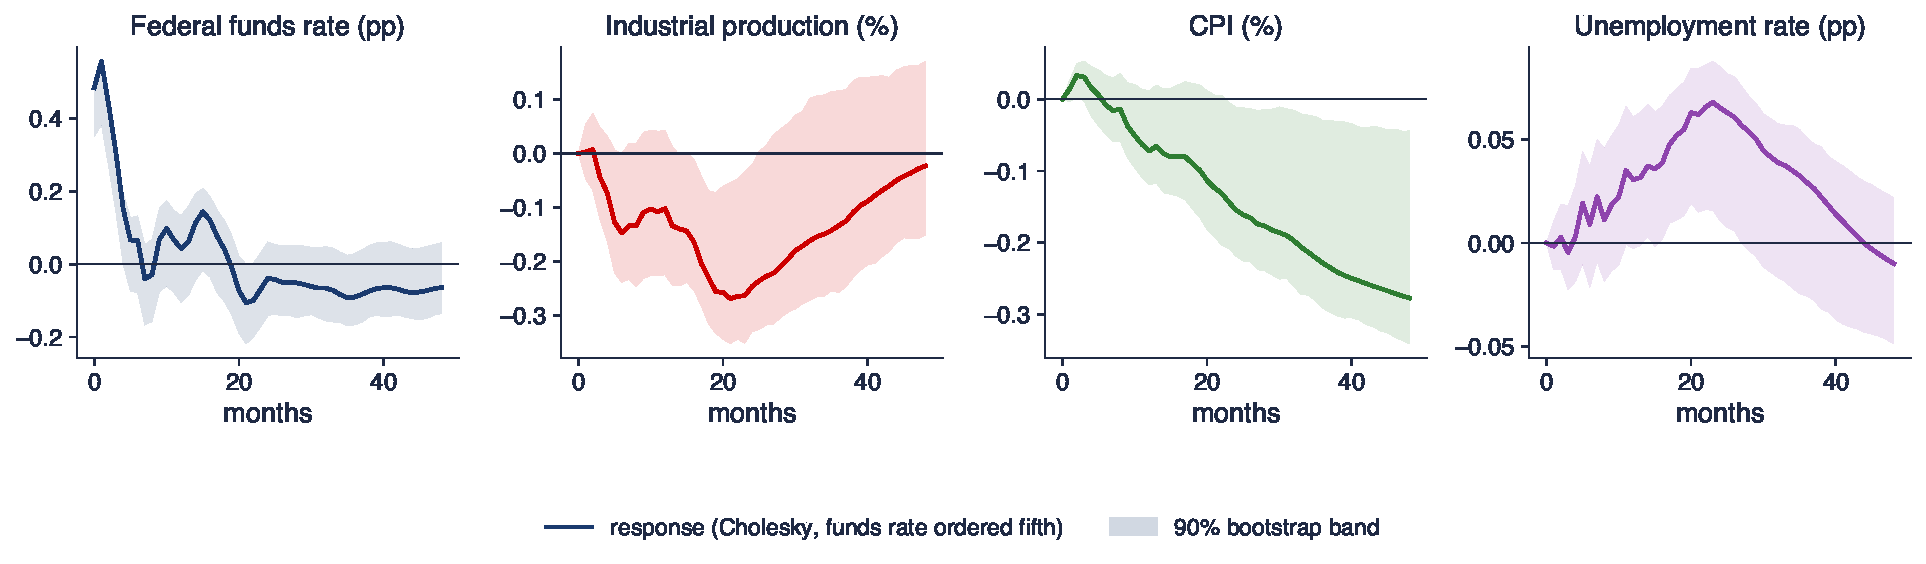
\includegraphics[width=0.97\textwidth,height=0.54\textheight,keepaspectratio]{ats_ch3_cee_irf.pdf}
\end{center}
\vspace{-0.25cm}
\begin{itemize}
    \item Responses to a one-standard-deviation funds-rate shock (0.48 pp); 90\% residual-bootstrap bands
\end{itemize}
\quantlet{ATS\_ch3\_recursive\_var}{\qlurl{ATS_ch3_recursive_var}}
\end{frame}

\begin{frame}{Interpreting the CEE responses}
\itemsize{\small}
\begin{itemize}
    \item Industrial production falls slowly: trough \ensuremath{-}0.27\% after 21 months (band [\ensuremath{-}0.35, \ensuremath{-}0.05]); unemployment rises by up to 0.07 pp
    \begin{itemize}
        \item the hump shape and the delay are the classic ``long and variable lags'' of monetary policy
    \end{itemize}
    \item Prices first rise slightly (0.033\% after 2 months), then fall to \ensuremath{-}0.28\% after four years
    \begin{itemize}
        \item the initial rise is the \textbf{price puzzle}: the Fed tightens when it expects inflation; commodity prices in the VAR reduce but do not remove it
    \end{itemize}
    \item Monetary shocks explain little of output: 6.6\% of the 24-month forecast error variance of IP
\end{itemize}
\end{frame}

\begin{frame}{Non-recursive short-run restrictions}
\itemsize{\small}
\begin{itemize}
    \item \textbf{AB model} \refLut, \refKL: $Au_t = B\varepsilon_t$; zeros and known values anywhere in $A$ and $B$
    \begin{itemize}
        \item $A$: the contemporaneous relations among $u_t$; $B$: the impact of the shocks; then $\Sigma_u = A^{-1}BB'A^{-1\prime}$
        \item estimated by maximum likelihood: maximise $-\frac T2\ln|\Sigma_u(A, B)| - \frac T2\mathrm{tr}[\Sigma_u(A, B)^{-1}\hat\Sigma_u]$
        \item $|\cdot|$: the determinant; $\mathrm{tr}$: the trace; $\hat\Sigma_u$: the residual covariance matrix of the reduced form
        \item over-identifying restrictions can be tested by a likelihood-ratio test against the just-identified model
    \end{itemize}
    \item \textbf{Blanchard--Perotti} \refBP: the automatic response of taxes to output is an \emph{external} elasticity (from tax codes)
    \begin{itemize}
        \item with that elasticity fixed, the cyclically adjusted tax innovation is an instrument for the remaining coefficients
        \item government spending is predetermined within the quarter (decision lags): a zero restriction with an institutional argument
    \end{itemize}
    \item Seminar 3, A2: one known elasticity identifies a $2\times2$ system by instrumental variables
\end{itemize}
\end{frame}

\begin{frame}{Limits of the recursive assumption}
\itemsize{\small}
\begin{itemize}
    \item Simultaneity: interest rates and asset prices react to each other within the day
    \begin{itemize}
        \item no ordering of stock prices and the policy rate is credible at a monthly frequency
    \end{itemize}
    \item Omitted information: the policy shock absorbs the Fed's forecasts
    \begin{itemize}
        \item narrative shocks \refRR\ purge the intended rate change of the Greenbook forecasts
    \end{itemize}
    \item Sample dependence: the post-1983 responses are weaker and often puzzling \refRam
    \begin{itemize}
        \item the remedies of the next sections: weaker restrictions (signs) or outside information (instruments)
    \end{itemize}
\end{itemize}
\end{frame}

\begin{frame}{Recap: Short-run restrictions}
\itemsize{\small}
\begin{itemize}
    \item Cholesky = timing assumptions; only the position of the shock variable matters for its responses
    \item CEE: output falls with a lag of about 21 months; the price puzzle remains
    \item Non-recursive schemes use institutional knowledge (tax elasticities, decision lags) and can be over-identified and tested
    \item Short-run zeros are least credible exactly where they matter most: fast markets
\end{itemize}
\end{frame}


%=============================================================================
\section{Case study: oil supply and demand shocks}
%=============================================================================

\begin{frame}{Not all oil price shocks are alike}
\itemsize{\footnotesize}
\begin{columns}[T]
\begin{column}{0.38\textwidth}
\centering
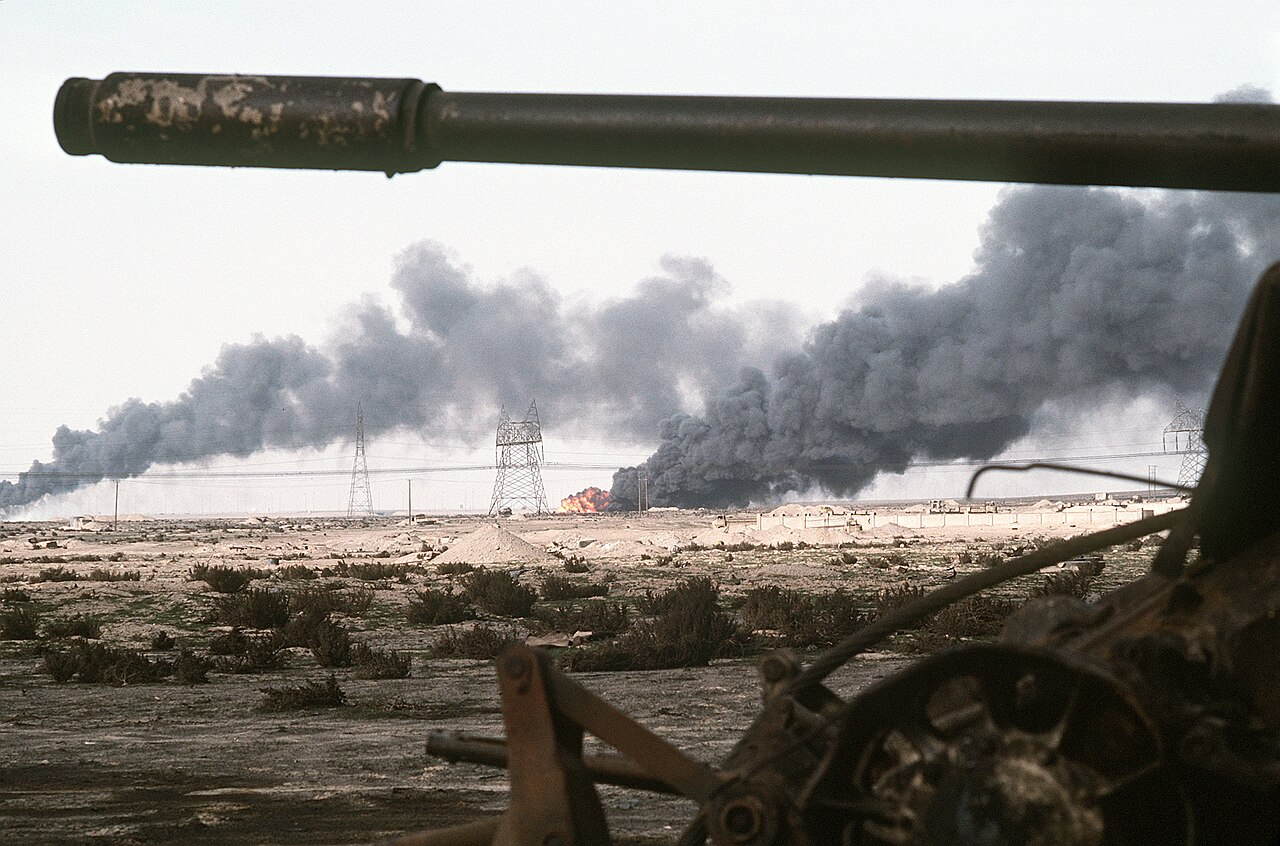
\includegraphics[height=0.36\textheight]{ch3_kuwait_oil_fires_1991.jpg}\\[1mm]
\imgcap{Burning Kuwaiti oil field, March 1991}
\imgcredit{https://commons.wikimedia.org/wiki/File:Disabled_Iraqi_T-54A,_T-55,_Type_59_or_Type_69_tank_and_burning_Kuwaiti_oil_field.jpg}{Photo: JO1 Gawlowicz, US Navy (1991); public domain; Wikimedia Commons}
\end{column}
\begin{column}{0.60\textwidth}
\begin{itemize}
    \item \refKilB: monthly VAR(24) in (i) the percent change of world crude oil production, (ii) global real activity, (iii) the log real price of oil
    \begin{itemize}
        \item recursive: oil supply does not respond within the month to demand (adjustment costs); real activity does not respond within the month to oil-specific demand
    \end{itemize}
    \item Three shocks: oil supply, aggregate demand, oil-specific (precautionary) demand
    \begin{itemize}
        \item real activity: the index of \refKilB\ as corrected in \refKilC\ (FRED IGREA); price: refiner acquisition cost of imported crude, deflated by the US CPI
    \end{itemize}
    \item Our sample starts in 1974 (first month of the price series), effective sample from January 1976, $T = 384$; extension to May 2026
\end{itemize}
\end{column}
\end{columns}
\end{frame}

\begin{frame}{Responses to oil supply and demand shocks}
\itemsize{\footnotesize}
\begin{center}
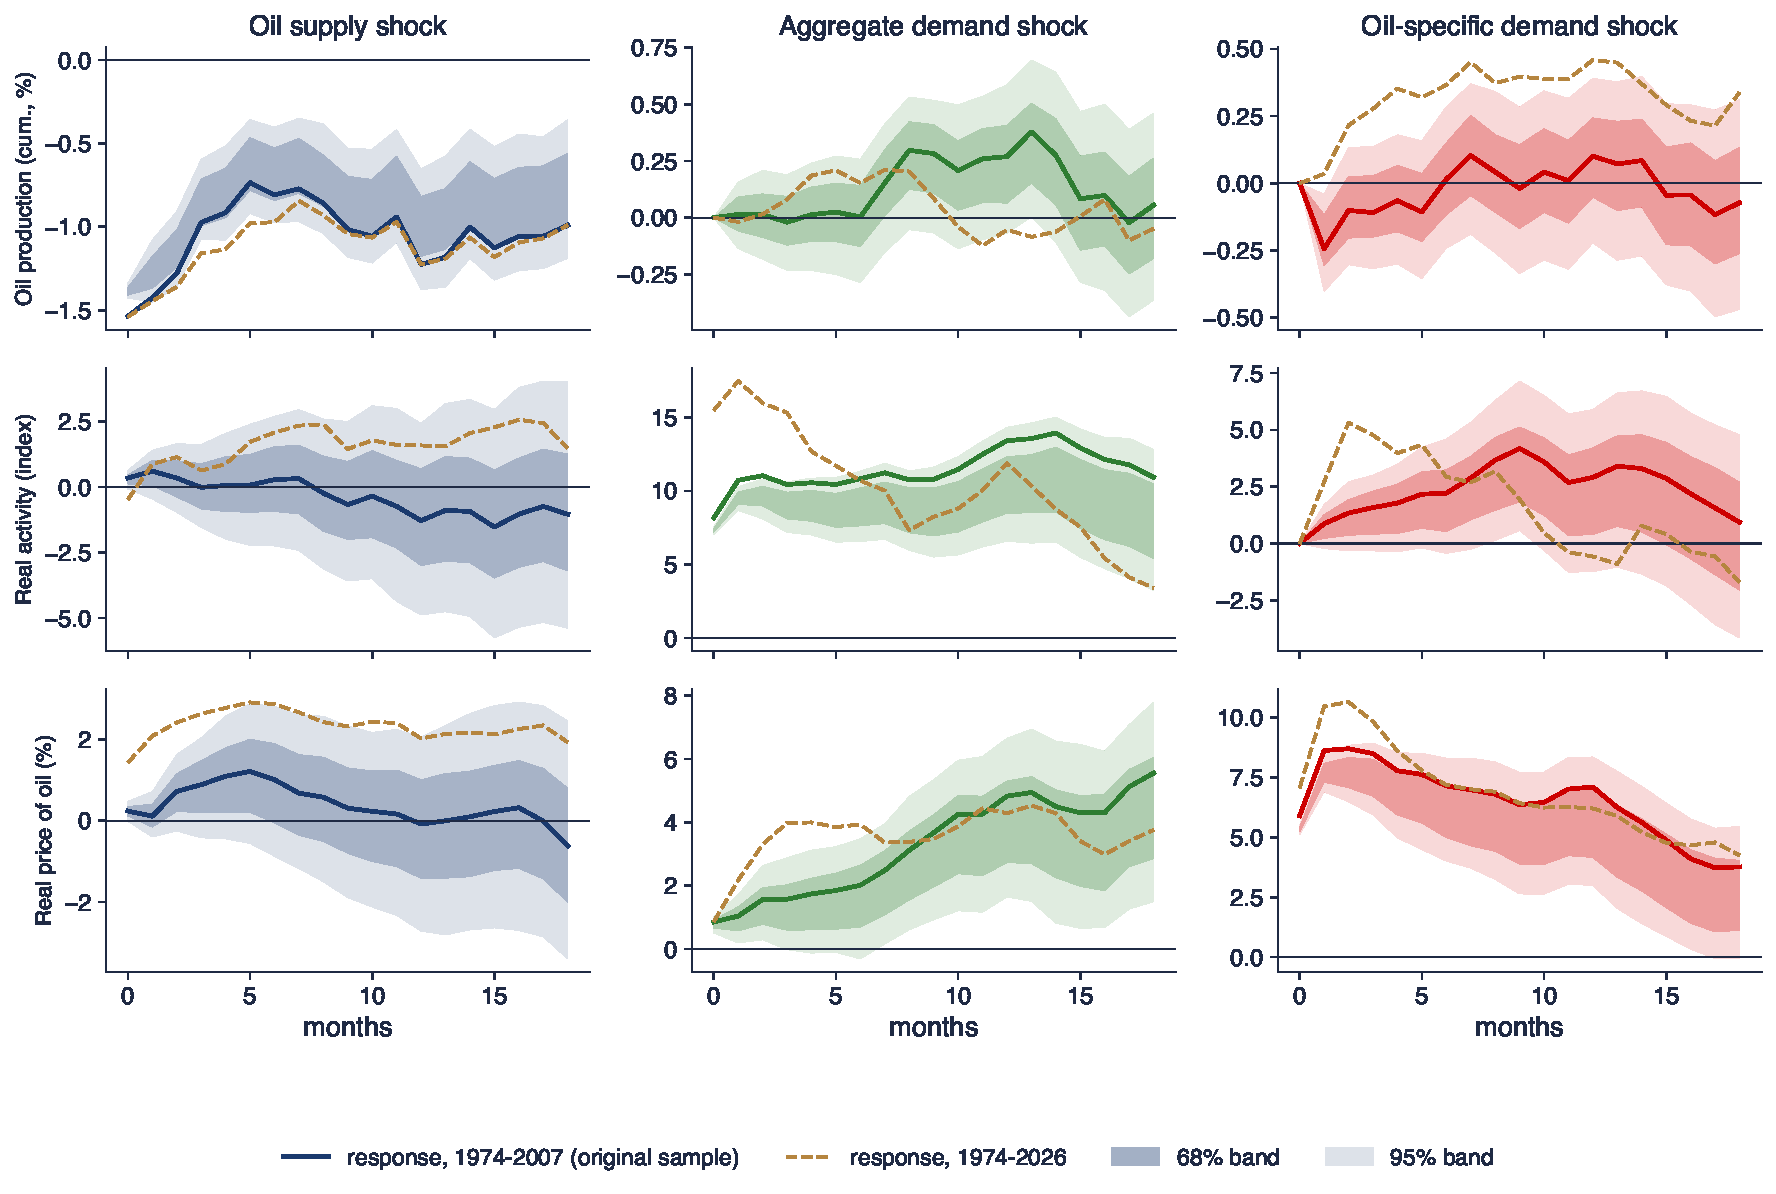
\includegraphics[width=0.97\textwidth,height=0.64\textheight,keepaspectratio]{ats_ch3_kilian_irf.pdf}
\end{center}
\vspace{-0.25cm}
\begin{itemize}
    \item One-standard-deviation shocks, production cumulated; 68\% and 95\% recursive-design wild-bootstrap bands \refGoK; dashed: sample extended to 2026
\end{itemize}
\quantlet{ATS\_ch3\_oil\_shocks}{\qlurl{ATS_ch3_oil_shocks}}
\end{frame}

\begin{frame}{Interpreting the oil responses}
\itemsize{\small}
\begin{itemize}
    \item Supply shock: production falls by \ensuremath{-}1.5\% on impact, the real price barely moves (\ensuremath{-}0.1\% after 12 months, band [\ensuremath{-}2.8, 2.2])
    \begin{itemize}
        \item in the extended sample the effect is larger (2.0\%): the post-2008 market reacts more to supply news
    \end{itemize}
    \item Aggregate demand: a delayed, persistent rise of the price (4.8\% after 12 months, band [1.5, 6.8])
    \item Oil-specific demand: an immediate jump (5.9\%) that persists (7.1\% after 12 months)
    \item At 60 months, supply shocks explain 1\% of the price variance, aggregate demand 64\%, oil-specific demand 35\%: oil prices are mostly demand-driven
\end{itemize}
\end{frame}

\begin{frame}{Historical decomposition of the real price of oil}
\itemsize{\footnotesize}
\begin{center}
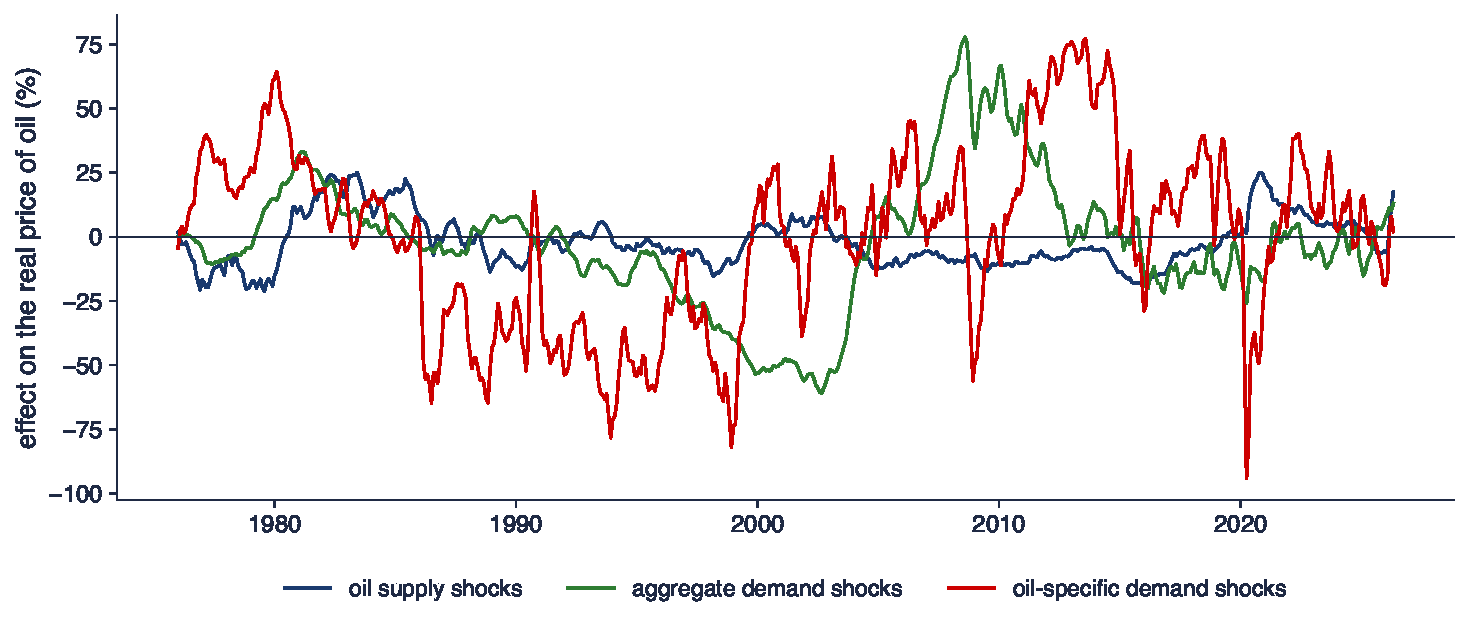
\includegraphics[width=0.97\textwidth,height=0.69\textheight,keepaspectratio]{ats_ch3_kilian_hd.pdf}
\end{center}
\vspace{-0.25cm}
\begin{itemize}
    \item Cumulative contribution of each structural shock, 1976--2026 (recursive VAR(24), extended sample); log points $\times 100$
\end{itemize}
\quantlet{ATS\_ch3\_oil\_shocks}{\qlurl{ATS_ch3_oil_shocks}}
\end{frame}

\begin{frame}{Interpreting the historical decomposition}
\itemsize{\small}
\begin{itemize}
    \item 2003--mid-2008: aggregate demand adds 126 log points, supply \ensuremath{-}12: the boom was a global demand boom
    \item Mid-2008 to early 2009: oil-specific demand \ensuremath{-}82, aggregate demand \ensuremath{-}35; early 2020: oil-specific demand \ensuremath{-}103
    \item Mid-2021 to mid-2022: oil-specific demand 43, supply \ensuremath{-}2: the model reads the 2022 surge as precautionary demand
    \item Caveat: the zero restriction on the supply response is strong; \refBHb\ allow a small but non-zero elasticity and find a larger role for supply
    \begin{itemize}
        \item a decomposition is only as good as the identifying assumption behind it
    \end{itemize}
\end{itemize}
\end{frame}


%=============================================================================
\section{Long-run restrictions}
%=============================================================================

\begin{frame}{Blanchard and Quah: the long-run multiplier (1/2)}
\itemsize{\small}
\begin{itemize}
    \item For $y_t = (\Delta\text{output}_t, u_t)'$ the cumulative responses are
    \begin{itemize}
        \item $\Theta(1) = \sum_h\Theta_h = (I - A_1 - \dots - A_p)^{-1}B_0 = A(1)^{-1}B_0$
        \item here $u_t$ is the unemployment rate; $A(1) = I - A_1 - \dots - A_p$: the VAR polynomial at 1; the first row of $\Theta(1)$ is the long-run effect on the \emph{level} of output
    \end{itemize}
    \item Restriction \refBQ: demand shocks have no long-run effect on the level of output
    \begin{itemize}
        \item $[\Theta(1)]_{12} = 0$
        \item $[\cdot]_{12}$: the element in row 1 (output) and column 2 (the demand shock)
    \end{itemize}
\end{itemize}
\end{frame}

\begin{frame}{Blanchard and Quah: the long-run multiplier (2/2)}
\itemsize{\small}
\begin{itemize}
    \item Algorithm: $\Theta(1)\Theta(1)' = A(1)^{-1}\Sigma_uA(1)^{-1\prime}$ is known from the reduced form
    \begin{itemize}
        \item take its lower-triangular Cholesky factor $L$ (the zero in position $(1,2)$), then $B_0 = A(1)L$
        \item the zero is placed on the long-run matrix, not on the impact matrix; derivation in the \atsapplink{atsapp1}{atssrc1}{Appendix} and in Seminar 3, A3
    \end{itemize}
    \item Interpretation: ``supply'' = all shocks with permanent effects (technology, labour supply); \refGali\ uses the same idea for technology shocks and hours
\end{itemize}
\end{frame}

\begin{frame}{Case study: Blanchard and Quah (1989)}
\itemsize{\small}
\begin{itemize}
    \item The paper: US real GNP growth and the unemployment rate (men aged 20 and over), quarterly, VAR(8), 1950:2--1987:4 \refBQ
    \begin{itemize}
        \item data treatment: separate means of output growth before and after 1973:4 (the productivity slowdown), a linear trend removed from unemployment
    \end{itemize}
    \item Our replication: the same specification on today's vintage (FRED GNPC96, LNS14000025), $T = 151$; 90\% residual-bootstrap bands
    \item Question: do demand shocks drive the business cycle, and how long do their effects last?
\end{itemize}
\end{frame}

\begin{frame}{Supply and demand shocks identified by a long-run restriction}
\itemsize{\footnotesize}
\begin{center}
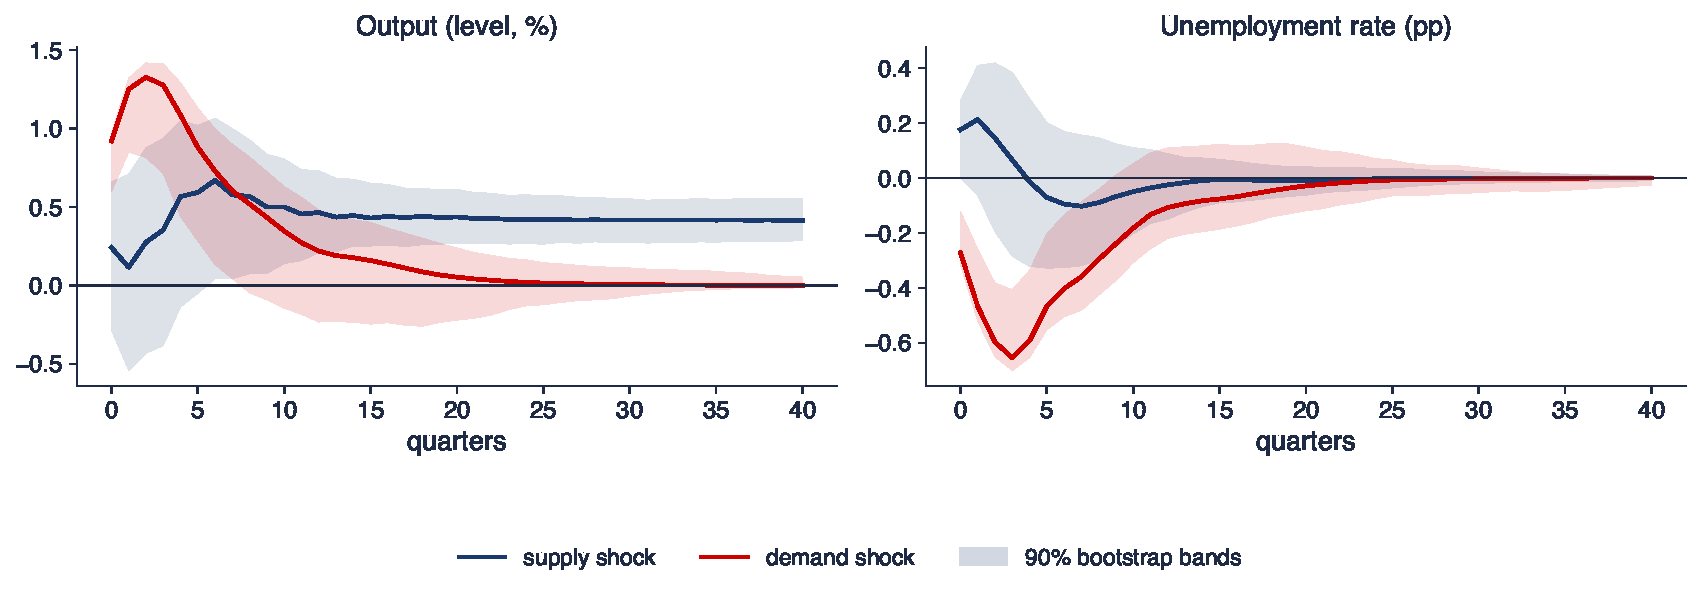
\includegraphics[width=0.97\textwidth,height=0.65\textheight,keepaspectratio]{ats_ch3_bq.pdf}
\end{center}
\vspace{-0.25cm}
\begin{itemize}
    \item Output level (cumulated growth) and unemployment; one-standard-deviation shocks; 90\% bootstrap bands
\end{itemize}
\quantlet{ATS\_ch3\_long\_run}{\qlurl{ATS_ch3_long_run}}
\end{frame}

\begin{frame}{Interpreting the Blanchard--Quah responses}
\itemsize{\small}
\begin{itemize}
    \item Demand shock: output peaks at 1.33\% after 2 quarters and returns to zero by construction; unemployment falls by \ensuremath{-}0.65 pp
    \item Supply shock: output rises permanently (0.42\% after ten years, band [0.28, 0.55]), unemployment first \emph{rises} (0.18 pp)
    \item Demand shocks explain 92\% of the output-level variance at one year and 54\% at ten years: in line with \refBQ, demand dominates at business-cycle horizons
    \item Seminar 3, B5: without the break and the trend, the shares change dramatically
\end{itemize}
\end{frame}

\begin{frame}{Reliability of long-run restrictions}
\itemsize{\small}
\begin{itemize}
    \item \refFL: the long-run multiplier $A(1)^{-1}$ is estimated imprecisely from finite samples
    \begin{itemize}
        \item a shock with a tiny but permanent effect is indistinguishable from a transitory one: inference can be arbitrarily distorted
        \item the near-unit-root behaviour of unemployment makes the problem worse
    \end{itemize}
    \item Results depend on the treatment of low frequencies: breaks in mean growth, trends, the lag length
    \begin{itemize}
        \item \atschlink{https://danpele.github.io/Advanced-Time-Series/EN/Courses/chapter2_structural_breaks_nonlinear_models.pdf}{Chapter 2} tests for such breaks; \atschlink{https://danpele.github.io/Advanced-Time-Series/EN/Courses/chapter4_cointegration_vecm_ardl_panel.pdf}{Chapter 4} treats cointegration, where long-run restrictions become restrictions on the VECM
    \end{itemize}
    \item Use long-run restrictions with a sensitivity table, never alone
\end{itemize}
\end{frame}

\begin{frame}{Recap: Long-run restrictions}
\itemsize{\small}
\begin{itemize}
    \item Restrict $\Theta(1) = A(1)^{-1}B_0$ instead of $B_0$: identification from permanence
    \item BQ: demand dominates business-cycle fluctuations in output, supply the long run
    \item Fragile: low-frequency treatment and the imprecise long-run multiplier drive the answer
\end{itemize}
\end{frame}


%=============================================================================
\section{Sign restrictions and set identification}
%=============================================================================

\begin{frame}{Identification by signs (1/2)}
\itemsize{\small}
\begin{itemize}
    \item Restrict only the \textbf{signs} of some responses for some horizons: a contractionary monetary shock raises the rate and lowers prices \refUhl
    \begin{itemize}
        \item the response of interest (output) is left unrestricted: an ``agnostic'' procedure
    \end{itemize}
    \item Algorithm \refRWZ: draw a random rotation $Q$
    \begin{itemize}
        \item draw $X$ ($n \times n$) with i.i.d.\ $N(0, 1)$ entries and compute its QR decomposition $X = QR$ ($Q$ orthogonal, $R$ upper triangular)
        \item normalise the signs of $\mathrm{diag}(R)$ to be positive: then $Q$ is uniform (Haar) on the set of orthogonal matrices
    \end{itemize}
\end{itemize}
\end{frame}

\begin{frame}{Identification by signs (2/2)}
\itemsize{\small}
\begin{itemize}
    \item Accept or reject the rotation
    \begin{itemize}
        \item compute $\Theta_h = \Phi_hPQ$ and keep $Q$ if all signs hold; repeat for draws of $(A, \Sigma_u)$ from the posterior
        \item zero restrictions together with signs need the importance-sampling algorithm of \refARW
    \end{itemize}
    \item The result is a \textbf{set} of models consistent with the data and the restrictions, not a point
\end{itemize}
\end{frame}

\begin{frame}{Sign restrictions in two dimensions}
\itemsize{\footnotesize}
\begin{center}
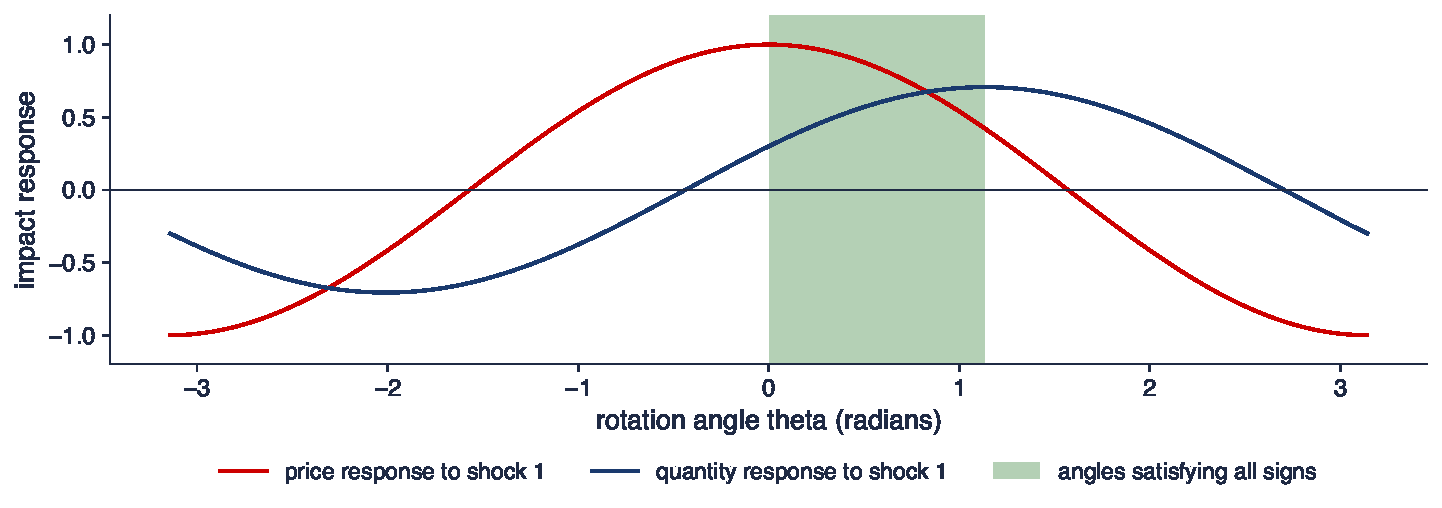
\includegraphics[width=0.97\textwidth,height=0.65\textheight,keepaspectratio]{ats_ch3_rotation.pdf}
\end{center}
\vspace{-0.25cm}
\begin{itemize}
    \item Price and quantity innovations with variances 1 and 0.5 and covariance 0.3; impact responses $P(\cos\theta, \sin\theta)'$ to shock 1 as the rotation angle varies; demand: $(+, +)$, supply: $(+, -)$
\end{itemize}
\quantlet{ATS\_ch3\_sign\_restrictions}{\qlurl{ATS_ch3_sign_restrictions}}
\end{frame}

\begin{frame}{Interpreting the rotation set}
\itemsize{\small}
\begin{itemize}
    \item All signs hold for $\theta \in (0, 1.13)$, 18\% of the circle: a whole interval of models is equally consistent with the data
    \item The impact effect of demand on quantity lies anywhere in $[0.30, 0.71]$: the \textbf{identified set}
    \item A uniform draw of $\theta$ puts a prior on this interval: the posterior inside the set is the prior, not information from data
    \begin{itemize}
        \item this is the point of \refBHa: Haar draws are informative about the responses
    \end{itemize}
\end{itemize}
\end{frame}

\begin{frame}{Case study: Uhlig (2005)}
\itemsize{\small}
\begin{itemize}
    \item The paper: six-variable monthly US VAR(12), no constant, 1965:1--2003:12; a contractionary shock raises the funds rate and lowers prices, commodity prices and nonborrowed reserves for months 0--5 \refUhl
    \begin{itemize}
        \item output is not restricted: the question is its sign
    \end{itemize}
    \item Our replication: the same restrictions and sample; IP and CPI replace the interpolated monthly GDP and deflator of the paper (data of \refRam)
    \begin{itemize}
        \item flat Normal--inverse-Wishart posterior, 1\,000 draws, Haar impulse vectors; accepted: 985 draws; at the OLS estimate 4.1\% of rotations satisfy the signs
    \end{itemize}
    \item Question: does a contractionary monetary shock lower output when output is left free?
\end{itemize}
\end{frame}

\begin{frame}{An agnostic monetary policy shock}
\itemsize{\footnotesize}
\begin{center}
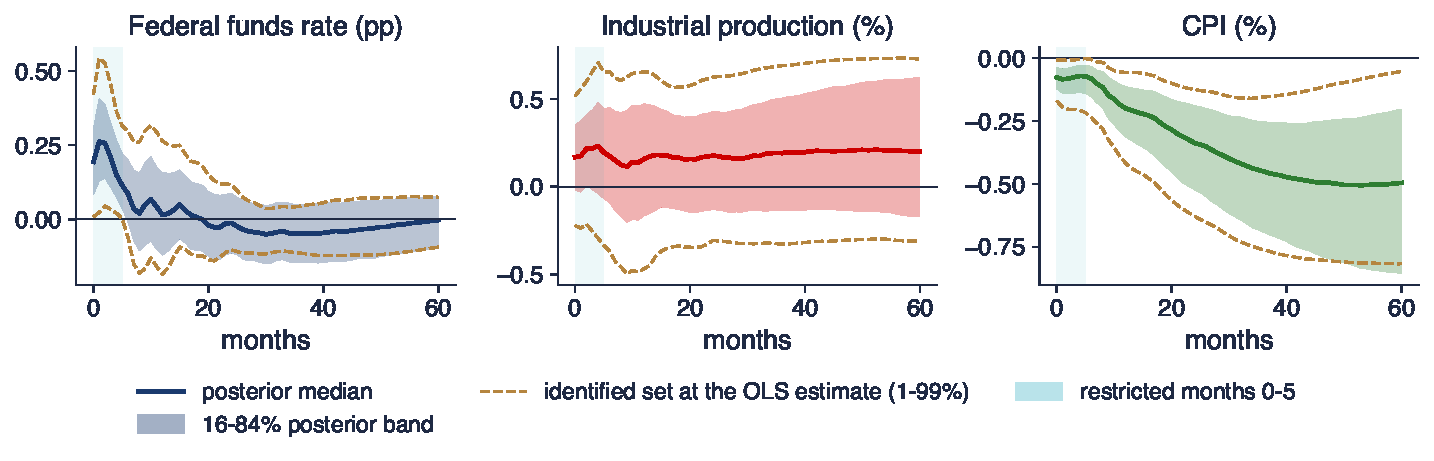
\includegraphics[width=0.97\textwidth,height=0.59\textheight,keepaspectratio]{ats_ch3_uhlig.pdf}
\end{center}
\vspace{-0.25cm}
\begin{itemize}
    \item One-standard-deviation shock; posterior median and 16--84\% band; dashed: 1--99\% range of the identified set at the OLS estimate; shaded: restricted months
\end{itemize}
\quantlet{ATS\_ch3\_sign\_restrictions}{\qlurl{ATS_ch3_sign_restrictions}}
\end{frame}

\begin{frame}{Interpreting the agnostic responses}
\itemsize{\small}
\begin{itemize}
    \item Output after 12 months: median 0.16\%, band [\ensuremath{-}0.17, 0.47]; 32\% of draws negative: no evidence that output falls
    \item The identified set at the OLS estimate spans [\ensuremath{-}0.47, 0.66]: the data with the signs cannot sign output
    \item Prices fall persistently (\ensuremath{-}0.34\% after 24 months) without a price puzzle, because the restriction rules it out
    \item Uhlig's conclusion, confirmed: neutrality of monetary policy shocks for output is not inconsistent with the data
\end{itemize}
\end{frame}

\begin{frame}{Inference under set identification}
\itemsize{\small}
\begin{itemize}
    \item The posterior median is not a structural model: at each horizon it can come from a different rotation \refFP
    \begin{itemize}
        \item report a single admissible model close to the median (median target) or, better, the whole set
    \end{itemize}
    \item The Haar prior is informative about the responses \refBHa; \refGKi\ propose robust Bayes: report the range of posterior means over all priors on $Q$
    \begin{itemize}
        \item the robust band is wider and honest: it separates what the data say from what the prior says
    \end{itemize}
    \item Tighten the set with more information: more signs, zeros \refARW, narrative events, elasticity bounds \refBHb
\end{itemize}
\end{frame}

\begin{frame}{Narrative restrictions}
\itemsize{\footnotesize}
\begin{columns}[T]
\begin{column}{0.36\textwidth}
\centering

\includegraphics[height=0.34\textheight]{ch3_volcker_2014.jpg}\\[1mm]
\imgcap{Paul Volcker, Fed Chairman 1979--1987}
\imgcredit{https://commons.wikimedia.org/wiki/File:Paul_Volcker_-_2014_(13896577879)_(cropped).jpg}{Photo: Federal Reserve (2014); public domain; Wikimedia Commons}
\end{column}
\begin{column}{0.62\textwidth}
\begin{itemize}
    \item \refADRR: restrict the structural shocks at specific dates, not the responses
    \begin{itemize}
        \item October 1979 (the Volcker shift to reserve targeting) was a positive monetary policy shock
        \item and it was the main contributor to the unexpected change of the funds rate that month
    \end{itemize}
    \item A few credible events remove most of the rotations that sign restrictions alone leave
    \begin{itemize}
        \item the likelihood must be reweighted by the probability of satisfying the narrative (importance sampling)
    \end{itemize}
    \item With narrative restrictions output falls after a contractionary shock, unlike in the agnostic set
\end{itemize}
\end{column}
\end{columns}
\end{frame}

\begin{frame}{Identification through heteroskedasticity}
\itemsize{\small}
\begin{itemize}
    \item If the variances of the structural shocks change across regimes while $B_0$ stays fixed: $\Sigma_1 = B_0B_0'$, $\Sigma_2 = B_0\Lambda B_0'$, $\Lambda$ diagonal \refRig
    \begin{itemize}
        \item $\Sigma_1, \Sigma_2$: the reduced-form covariance matrices of the two regimes; $\Lambda = \mathrm{diag}(\lambda_1, \dots, \lambda_n)$: the relative variances of the shocks in regime 2
        \item then $\Sigma_1^{-1}\Sigma_2 = B_0^{-1\prime}\Lambda B_0'$: the columns of $B_0$ follow from an eigendecomposition, unique if the $\lambda_i$ are distinct
        \item regimes: known dates (crises, policy announcements) or estimated (Markov switching, GARCH) \refLL
    \end{itemize}
    \item Statistical identification gives shocks without names: labelling them still needs economics (signs)
    \begin{itemize}
        \item the assumption that $B_0$ is the same in both regimes is strong and testable only partly
    \end{itemize}
    \item Seminar 3, A8 recovers $B_0$ from two covariance matrices by hand; \atschlink{https://danpele.github.io/Advanced-Time-Series/EN/Courses/chapter7_regime_switching_models.pdf}{Chapter 7} develops regime switching
\end{itemize}
\end{frame}

\begin{frame}{Recap: Sign restrictions and set identification}
\itemsize{\small}
\begin{itemize}
    \item Signs give a set of models; report the set, not only the posterior median
    \item Uhlig: with prices, rates and reserves restricted, output can go either way
    \item The Haar prior matters; robust Bayes and narrative restrictions sharpen honest conclusions
    \item Heteroskedasticity identifies statistically; economics still names the shocks
\end{itemize}
\end{frame}


%=============================================================================
\section{External instruments}
%=============================================================================

\begin{frame}{The proxy SVAR (1/2)}
\itemsize{\small}
\begin{itemize}
    \item An external variable $z_t$ (the proxy), correlated with the shock of interest $\varepsilon_{1t}$ and with no other shock
    \begin{itemize}
        \item \textbf{relevance}: $\E z_t\varepsilon_{1t} = \alpha \ne 0$; \textbf{exogeneity}: $\E z_t\varepsilon_{jt} = 0$ for $j \ne 1$
    \end{itemize}
    \item Then the covariance of the residuals with the proxy is proportional to the impact column $b_1$
    \begin{itemize}
        \item $\E u_tz_t = B_0\E\varepsilon_tz_t = \alpha b_1$ (derivation in the \atsapplink{atsapp2}{atssrc2}{Appendix})
        \item $b_1$: the first column of $B_0$, the impact effects of shock 1 on all $n$ variables
    \end{itemize}
\end{itemize}
\end{frame}

\begin{frame}{The proxy SVAR (2/2)}
\itemsize{\small}
\begin{itemize}
    \item Normalise $b_{11} = 1$ (or a 25 bp rate increase) and estimate the relative impacts \refSWb, \refMR
    \begin{itemize}
        \item $b_{i1}/b_{11} = \E(u_{it}z_t)/\E(u_{1t}z_t)$
        \item $b_{i1}$: the impact on variable $i$; numerically a 2SLS regression of $u_{it}$ on $u_{1t}$ with instrument $z_t$
    \end{itemize}
    \item Responses $\Theta_{h,\cdot1} = \Phi_hb_1$: the first column of $\Theta_h$
    \begin{itemize}
        \item the proxy may be noisy, short or available only for a sub-sample
    \end{itemize}
    \item Only one column of $B_0$ is identified, and no zero restriction is needed
\end{itemize}
\end{frame}

\begin{frame}{High-frequency identification of monetary policy}
\itemsize{\small}
\begin{itemize}
    \item Surprise = change of futures-implied rates in a narrow window (30 minutes) around an FOMC announcement \refKut, \refGSS
    \begin{itemize}
        \item within 30 minutes nothing else systematic happens: exogeneity by design
        \item FF4: the three-month-ahead federal funds futures; it captures forward guidance as well as the current decision \refGK
    \end{itemize}
    \item Complications: the \textbf{information effect} \refNS: a tightening can signal good news about the economy
    \begin{itemize}
        \item \refJK\ separate pure policy and information shocks with the co-movement of rates and stock prices (sign restrictions on surprises)
        \item surprises are predictable from past macro news \refBS: orthogonalise them before use
    \end{itemize}
\end{itemize}
\end{frame}

\begin{frame}{Case study: Gertler and Karadi (2015)}
\itemsize{\small}
\begin{itemize}
    \item The paper: the 1-year Treasury yield as policy indicator (it captures forward guidance), log IP, log CPI and the excess bond premium of \refGZ; VAR(12), 1979:7--2012:6 \refGK
    \begin{itemize}
        \item instrument: FF4 surprises, monthly, 1991:1--2012:6; the residuals of the full sample are used for the proxy regression on the overlap
    \end{itemize}
    \item Our replication: the same variables, sample and instrument (replication files of \refRam), $T = 384$, $258$ months with the instrument
    \begin{itemize}
        \item first stage: robust $F = 17.7$ (homoskedastic 21.9), $R^2 = 7.8\%$; 90\% moving-block bootstrap bands \refJL
    \end{itemize}
    \item Question: does a policy surprise move credit spreads, and with what effect on activity?
\end{itemize}
\end{frame}

\begin{frame}{A monetary policy shock identified with FF4 surprises}
\itemsize{\footnotesize}
\begin{center}
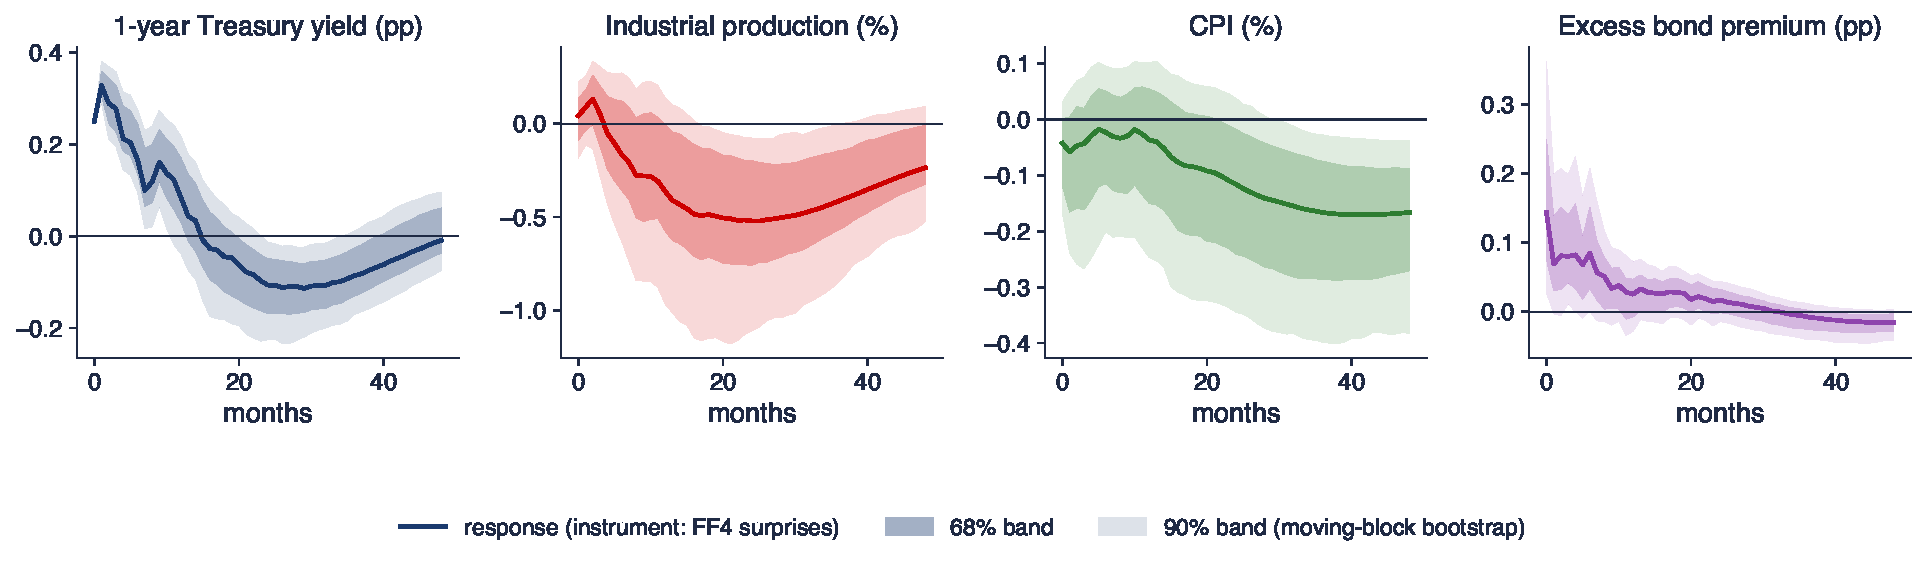
\includegraphics[width=0.97\textwidth,height=0.54\textheight,keepaspectratio]{ats_ch3_gk.pdf}
\end{center}
\vspace{-0.25cm}
\begin{itemize}
    \item Shock normalised to raise the 1-year yield by 25 bp on impact; 68\% and 90\% moving-block bootstrap bands
\end{itemize}
\quantlet{ATS\_ch3\_proxy\_svar}{\qlurl{ATS_ch3_proxy_svar}}
\end{frame}

\begin{frame}{Interpreting the proxy SVAR}
\itemsize{\small}
\begin{itemize}
    \item The excess bond premium jumps by 0.14 pp on impact (band [0.03, 0.35]): monetary policy works through credit costs, in line with \refGK
    \item IP reaches \ensuremath{-}0.52\% after 25 months (band [\ensuremath{-}1.05, \ensuremath{-}0.12]); CPI is \ensuremath{-}0.12\% after two years (band [\ensuremath{-}0.34, 0.04]), with no price puzzle
    \item $F = 17.7$ passes the rule of thumb $F > 10$, but the price response is imprecise: weak-instrument-robust bands are wider \refMSW
\end{itemize}
\end{frame}

\begin{frame}{Inference with an external instrument}
\itemsize{\small}
\begin{itemize}
    \item Weak instruments: when $\alpha$ is small, the ratio $\E(u_iz)/\E(u_1z)$ is badly estimated and delta-method bands undercover
    \begin{itemize}
        \item first-stage $F$: the $F$ statistic of the regression of $u_{1t}$ on $z_t$; it measures the strength of the instrument
    \end{itemize}
    \item Remedies
    \begin{itemize}
        \item \refMSW: Anderson--Rubin-type confidence sets, valid for any strength; they can be unbounded
        \item report the first-stage $F$ with HAC variance; the rule $F > 10$ is a heuristic, not a test
    \end{itemize}
    \item Bootstrap: the wild bootstrap of \refMR\ is invalid for proxy SVARs; use the moving-block bootstrap of residuals and instrument jointly \refJL
    \begin{itemize}
        \item the block keeps the dependence between the squared shock and the instrument
    \end{itemize}
    \item Seminar 3, A5 computes relative impacts and $F$ by hand; C1 builds an Anderson--Rubin set for Romania
\end{itemize}
\end{frame}

\begin{frame}{Recap: External instruments}
\itemsize{\small}
\begin{itemize}
    \item Relevance + exogeneity of a proxy identify one column of $B_0$, with no zeros
    \item High-frequency surprises are the best proxies we have; check the information effect and predictability
    \item GK replicated: credit spreads jump, output falls; $F = 17.7$
    \item Use weak-IV-robust sets and the block bootstrap
\end{itemize}
\end{frame}


%=============================================================================
\section{Inference for impulse responses}
%=============================================================================

\begin{frame}{Delta method and its limits}
\itemsize{\small}
\begin{itemize}
    \item $\hat\Theta_h = g(\hat\beta, \hat\sigma)$ is a smooth function of the VAR estimates: $\sqrt T(\hat\Theta_h - \Theta_h) \to N(0, G\Sigma G')$ \refLut
    \begin{itemize}
        \item $\hat\beta$: the VAR coefficients; $\hat\sigma$: the distinct elements of $\hat\Sigma_u$; $\Sigma$: their joint asymptotic covariance
        \item $G = \partial g/\partial(\beta, \sigma)$: the Jacobian, in closed form; quick, but the bands are symmetric
    \end{itemize}
    \item It fails where we need it most
    \begin{itemize}
        \item near unit roots and at long horizons the distribution of $\hat\Theta_h$ is skewed and non-Normal
        \item the covariance $G\Sigma G'$ can be singular (e.g.\ when a response is zero by construction)
        \item OLS slope estimates are biased towards zero in small samples, so responses decay too fast
    \end{itemize}
    \item Hence the bootstrap, and the bias correction
\end{itemize}
\end{frame}

\begin{frame}{Bootstrap schemes for VARs}
\itemsize{\small}
\begin{itemize}
    \item \textbf{Residual (recursive-design)}: resample $\hat u_t$ i.i.d., rebuild $y^*_t$ recursively from the estimated VAR, re-estimate, identify, repeat
    \begin{itemize}
        \item valid with i.i.d.\ innovations; the percentile (or Hall) interval of the $B$ responses gives the band
    \end{itemize}
    \item \textbf{Wild}: $u^*_t = \eta_t\hat u_t$, $\eta_t = \pm1$ with probability $1/2$: robust to conditional heteroskedasticity \refGoK
    \begin{itemize}
        \item used for the oil VAR: commodity markets have volatility clustering
    \end{itemize}
    \item \textbf{Moving block}: resample blocks of consecutive $(\hat u_t, z_t)$; needed whenever higher moments matter (proxy SVAR) \refJL
    \begin{itemize}
        \item block length of order $T^{1/4}$; \atschlink{https://danpele.github.io/Advanced-Time-Series/EN/Courses/chapter0_refresher_inference.pdf}{Chapter 0} covered the choice
    \end{itemize}
\end{itemize}
\end{frame}

\begin{frame}{Kilian's bias-corrected bootstrap}
\itemsize{\small}
\begin{itemize}
    \item \refKilA: (1) bootstrap the bias $\hat b = \bar A^* - \hat A$; (2) correct $\tilde A = \hat A - \hat b$, shrinking the correction if $\tilde A$ is not stationary; (3) bootstrap again from $\tilde A$ and correct each replicate
    \begin{itemize}
        \item $\hat A$: the OLS estimate of the VAR coefficients; $\bar A^*$: the mean of the bootstrap estimates; $\tilde A$: the bias-corrected estimate
        \item the ``bootstrap after bootstrap'' recentres the distribution where OLS bias is large: persistent series, short samples
    \end{itemize}
    \item Oil VAR: mean absolute bias 0.009 per coefficient; largest root 0.994 before, 0.9999 after the (shrunk) correction
    \begin{itemize}
        \item 12-month response of the price to oil-specific demand: 7.11\% (OLS), 7.34\% (corrected), band [3.4, 9.1]; to aggregate demand: 4.83\% and 4.95\%
    \end{itemize}
    \item The correction makes responses more persistent; when the VAR in levels has a root above one, the rule of Kilian leaves it uncorrected (Romanian VAR, Section 9)
\end{itemize}
\end{frame}

\begin{frame}{Pointwise and joint bands}
\itemsize{\small}
\begin{itemize}
    \item A pointwise 90\% band covers $\Theta_h$ at each $h$ separately; the whole path lies inside it with much lower probability
    \begin{itemize}
        \item questions about the \emph{shape} (``output falls for two years'') need simultaneous bands \refMOPa
        \item sup-$t$ band: scale the pointwise standard errors by the $1 - \alpha$ quantile of $\max_h|t_h|$ from the bootstrap
        \item $t_h$: the bootstrap response at horizon $h$ minus the estimate, over its standard error; $\max_h|t_h|$: the largest deviation along the whole path
    \end{itemize}
    \item Bayesian bands (posterior quantiles) answer a different question: probability statements given the prior
    \begin{itemize}
        \item \atschlink{https://danpele.github.io/Advanced-Time-Series/EN/Courses/chapter5_bvar_factor_models_nowcasting.pdf}{Chapter 5} builds them with Minnesota and Normal--inverse-Wishart priors; with set identification they mix prior and data (previous section)
    \end{itemize}
    \item Always state: pointwise or joint, frequentist or Bayesian, the level (68\%, 90\%, 95\%)
\end{itemize}
\end{frame}

\begin{frame}{Recap: Inference for impulse responses}
\itemsize{\small}
\begin{itemize}
    \item Delta-method bands are symmetric and fail near unit roots
    \item Residual, wild and block bootstraps match i.i.d., heteroskedastic and proxy settings
    \item Kilian's correction removes small-sample bias; it is not applied to explosive estimates
    \item Shape questions need joint bands; Bayesian bands come in \atschlink{https://danpele.github.io/Advanced-Time-Series/EN/Courses/chapter5_bvar_factor_models_nowcasting.pdf}{Chapter 5}
\end{itemize}
\end{frame}


%=============================================================================
\section{Local projections}
%=============================================================================

\begin{frame}{Local projections}
\itemsize{\small}
\begin{itemize}
    \item \refJorda: one regression per horizon, $y_{i,t+h} = \mu_h + \beta_hx_t + \gamma_h'w_t + \xi_{t+h}$, $h = 0, 1, \dots, H$
    \begin{itemize}
        \item $y_{i,t+h}$: variable $i$, $h$ periods after the shock; $\mu_h$: an intercept; $\xi_{t+h}$: the projection error; $H$: the longest horizon
        \item $x_t$: the shock (or the policy variable with controls $w_t$ that make it as good as random); $\hat\beta_h$ is the impulse response
        \item no iteration of a model: a misspecified dynamic does not compound across horizons
    \end{itemize}
    \item The error $\xi_{t+h}$ is serially correlated (an MA($h - 1$) at least): HAC standard errors with $h + 1$ lags, or
    \begin{itemize}
        \item \textbf{lag augmentation} \refMOPb: add one more lag of the controls and use Eicker--Huber--White errors; valid uniformly over persistence, even near a unit root
    \end{itemize}
    \item Flexible: nonlinear terms, state dependence, panel data, cumulative outcomes all enter as regressors
\end{itemize}
\end{frame}

\begin{frame}{LP and VAR estimate the same responses}
\itemsize{\small}
\begin{itemize}
    \item \refPW: in population, an LP with $p$ lags of all variables as controls and a VAR($p$) with the same ordering give \emph{identical} responses up to horizon $p$ (\atsapplink{atsapp3}{atssrc3}{Appendix})
    \begin{itemize}
        \item with unrestricted lags ($p \to \infty$) they coincide at all horizons: the choice is about estimation, not identification
        \item any VAR identification scheme (recursive, external instrument) has an LP counterpart, and vice versa
    \end{itemize}
    \item In finite samples they differ: the VAR extrapolates the first $p$ autocovariances, the LP uses the raw $h$-step covariance
    \begin{itemize}
        \item the next slide quantifies this
    \end{itemize}
\end{itemize}
\end{frame}

\begin{frame}{Bias and variance: LP against VAR (simulation)}
\itemsize{\footnotesize}
\begin{center}
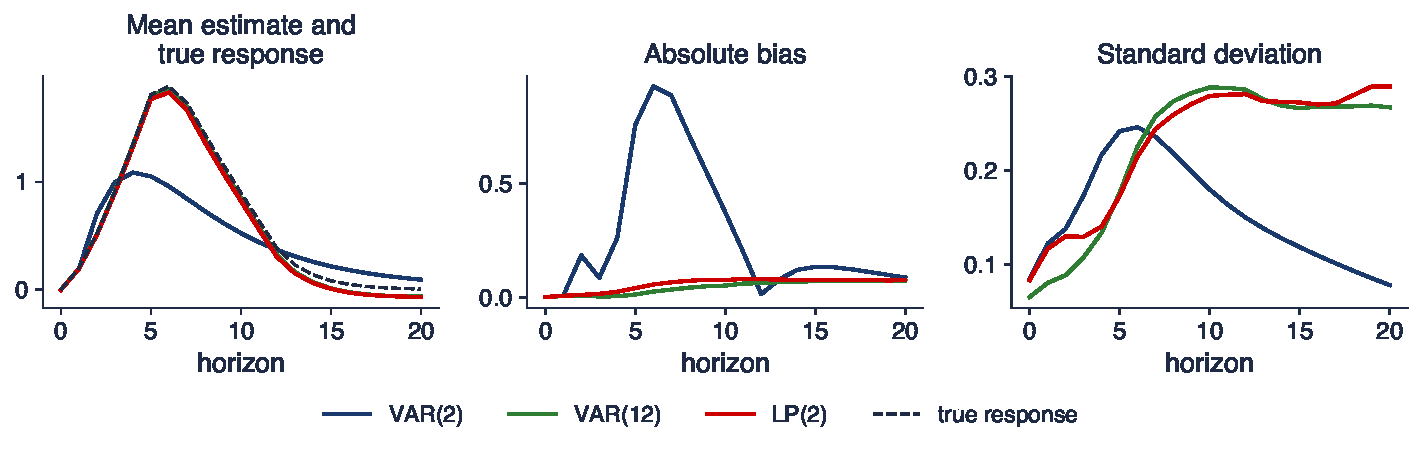
\includegraphics[width=0.97\textwidth,height=0.58\textheight,keepaspectratio]{ats_ch3_lp_sim.pdf}
\end{center}
\vspace{-0.25cm}
\begin{itemize}
    \item DGP: $x_t = 0.5x_{t-1} + e_t$, $y_t = 0.6y_{t-1} + \sum_{j=0}^{11}\psi_je_{t-j} + u_t$ (hump-shaped $\psi_j$), $T = 240$, 500 replications; $e_t, u_t$: independent white noises; a VAR(2) is misspecified
\end{itemize}
\quantlet{ATS\_ch3\_lp\_vs\_var}{\qlurl{ATS_ch3_lp_vs_var}}
\end{frame}

\begin{frame}{Interpreting the bias--variance trade-off}
\itemsize{\small}
\begin{itemize}
    \item At $h = 8$ (true response 1.44): VAR(2) bias 0.71, LP(2) bias 0.07; RMSE 0.74 and 0.27
    \begin{itemize}
        \item where the short VAR misses the hump, its bias dominates the error
    \end{itemize}
    \item At $h = 16$: standard deviation 0.11 (VAR(2)) against 0.27 (LP(2)); RMSE 0.17 against 0.28: the biased VAR wins
    \item The general lesson of \refLPW\ (thousands of DGPs): LP has low bias and high variance; VAR (and shrinkage VARs) have lower MSE unless the analyst cares almost only about bias
    \item A long VAR(12) behaves like LP: few lags = more bias, less variance
\end{itemize}
\end{frame}

\begin{frame}{LP-IV}
\itemsize{\small}
\begin{itemize}
    \item \refSWc: $y_{i,t+h} = \theta_{h,i}\,y_{1t} + \gamma'w_t + \xi_{t+h}$, with $y_{1t}$ (the policy rate) instrumented by $z_t$
    \begin{itemize}
        \item $\theta_{h,i}$ = response of $y_i$ after $h$ periods to a shock that raises $y_1$ by one unit on impact
        \item conditions: relevance, contemporaneous exogeneity and \textbf{lead-lag exogeneity} $\E z_t\varepsilon_{t+j} = 0$ for $j \ne 0$, given $w_t$
        \item lead-lag exogeneity: the instrument is unrelated to past and future shocks, not only to current ones
    \end{itemize}
    \item Same identifying information as the proxy SVAR; different estimator
    \begin{itemize}
        \item the proxy SVAR needs invertibility of the shock; LP-IV does not, but pays in variance
        \item cumulative LP-IV gives multipliers: $\sum_{j\le h}y_{t+j}$ on $\sum_{j\le h}g_{t+j}$ instrumented by $z_t$ \refRZ; $y$: output, $g$: government spending
    \end{itemize}
\end{itemize}
\end{frame}

\begin{frame}{The same instrument, two estimators}
\itemsize{\footnotesize}
\begin{center}
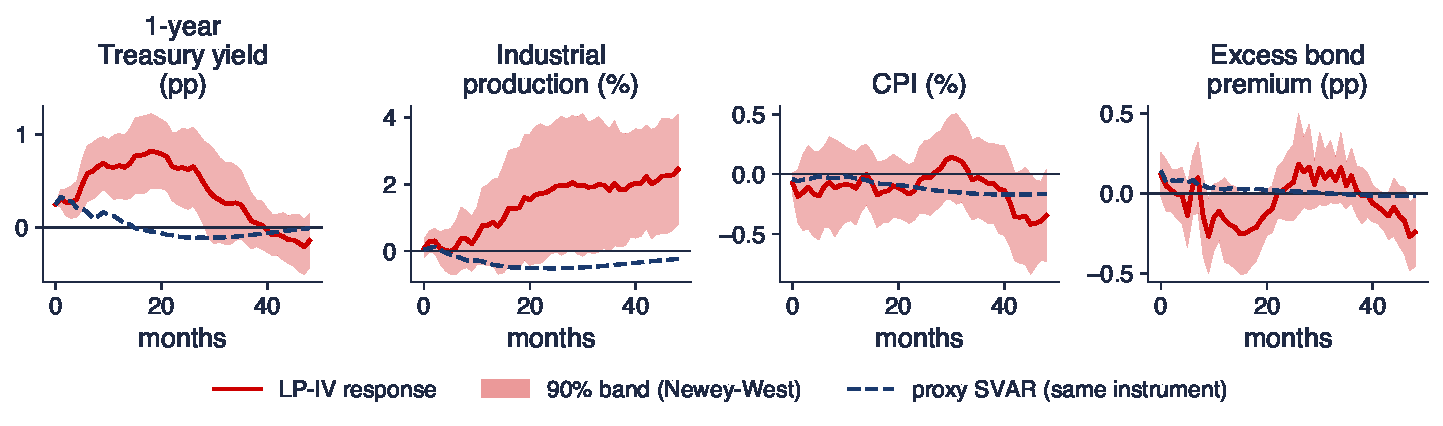
\includegraphics[width=0.97\textwidth,height=0.55\textheight,keepaspectratio]{ats_ch3_lp_gk.pdf}
\end{center}
\vspace{-0.25cm}
\begin{itemize}
    \item LP-IV with FF4 as instrument for the 1-year yield, 2 lags of all variables and of the instrument as controls, origins 1990:1--2012:6 ($T = 270$) \refRam; dashed: the proxy SVAR
\end{itemize}
\quantlet{ATS\_ch3\_lp\_vs\_var}{\qlurl{ATS_ch3_lp_vs_var}}
\end{frame}

\begin{frame}{Interpreting LP-IV against the proxy SVAR}
\itemsize{\small}
\begin{itemize}
    \item Impact first stage $F = 21.5$; after 24 months IP: LP-IV 1.84\% (SE 1.17), proxy SVAR \ensuremath{-}0.52\%
    \item CPI after 24 months: LP-IV \ensuremath{-}0.05\% (SE 0.17), proxy SVAR \ensuremath{-}0.12\%: the LP bands contain the VAR path almost everywhere
    \item LP-IV implies a much more persistent rise of the yield: the two estimators answer slightly different questions when the policy path differs
    \begin{itemize}
        \item the positive LP output response, noted by \refRam, is imprecise and sensitive to the sample: do not read it as expansionary tightening
    \end{itemize}
\end{itemize}
\end{frame}

\begin{frame}{State-dependent local projections (1/2)}
\itemsize{\small}
\begin{itemize}
    \item Interact everything with the state indicator of the previous period, $I_{t-1}$:
    \begin{itemize}
        \item $y_{t+h} = I_{t-1}[\alpha_{A,h} + \beta_{A,h}x_t + \dots] + (1 - I_{t-1})[\alpha_{B,h} + \beta_{B,h}x_t + \dots] + \xi_{t+h}$
        \item $I_{t-1} = 1$ in state A (e.g.\ slack), 0 in state B; $\beta_{A,h}$, $\beta_{B,h}$: the responses at horizon $h$ in each state; $\alpha$: state-specific intercepts
    \end{itemize}
    \item What LP measures here
    \begin{itemize}
        \item the state may change after the shock: LP measures the average response given the initial state, including transitions
        \item no need to model the state dynamics, unlike a threshold or a smooth-transition VAR (\atschlink{https://danpele.github.io/Advanced-Time-Series/EN/Courses/chapter2_structural_breaks_nonlinear_models.pdf}{Chapter 2})
    \end{itemize}
\end{itemize}
\end{frame}

\begin{frame}{State-dependent local projections (2/2)}
\itemsize{\small}
\begin{itemize}
    \item Case study \refRZ: are government spending multipliers larger in slack times?
    \begin{itemize}
        \item US quarterly data 1889--2015; military news shock (Ramey) scaled by potential GDP
        \item slack = unemployment $\ge 6.5\%$ in $t - 1$ (36\% of quarters)
        \item cumulative LP-IV of output on government spending, 4 lags of news, output and spending, Newey--West with $h + 1$ lags
    \end{itemize}
\end{itemize}
\end{frame}

\begin{frame}{Government spending multipliers by state of the economy}
\itemsize{\footnotesize}
\begin{center}
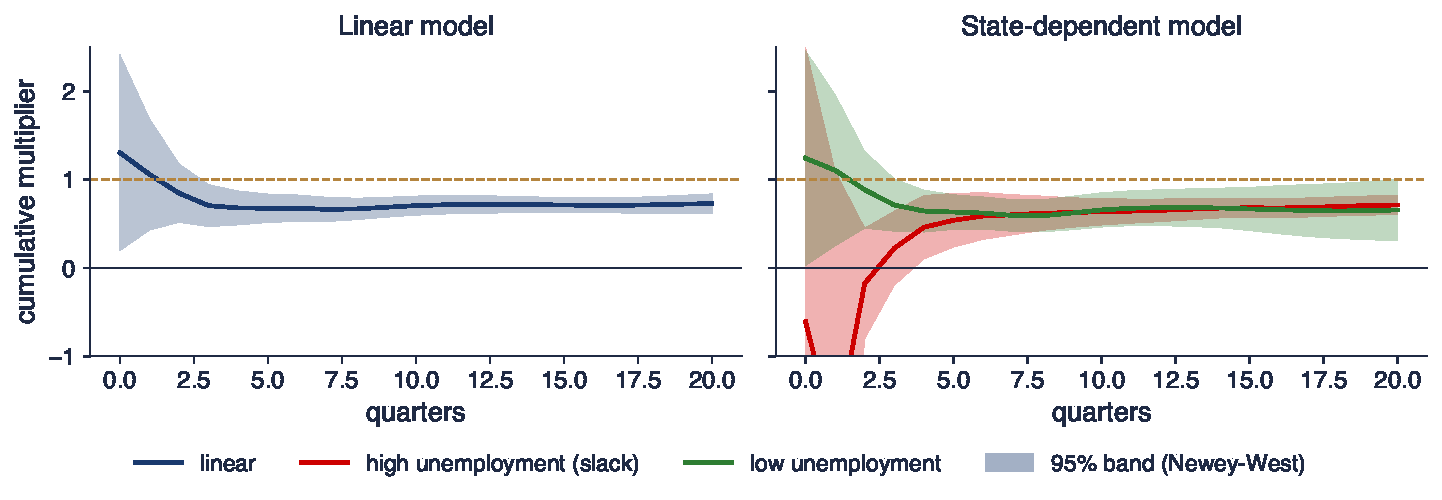
\includegraphics[width=0.97\textwidth,height=0.64\textheight,keepaspectratio]{ats_ch3_rz.pdf}
\end{center}
\vspace{-0.25cm}
\begin{itemize}
    \item Cumulative multiplier $\sum_{j\le h}\Delta y_{t+j}/\sum_{j\le h}\Delta g_{t+j}$ by horizon; 95\% Newey--West bands; dashed: multiplier of one
\end{itemize}
\quantlet{ATS\_ch3\_state\_dependent\_lp}{\qlurl{ATS_ch3_state_dependent_lp}}
\end{frame}

\begin{frame}{Interpreting the state-dependent multipliers}
\itemsize{\small}
\begin{itemize}
    \item Linear: 0.67 at two years (SE 0.06) and 0.71 at four years (SE 0.04)
    \item High unemployment: 0.62 and 0.68; low unemployment: 0.59 and 0.66
    \item In line with \refRZ: multipliers below one in both states and no significant difference between them
    \item The case for LP here: a VAR would impose the same dynamics in both states unless the state transitions are modelled
\end{itemize}
\end{frame}

\begin{frame}{Recap: Local projections}
\itemsize{\small}
\begin{itemize}
    \item LP = one regression per horizon; HAC or lag-augmented inference
    \item LP and VAR target the same responses; finite samples trade bias for variance
    \item LP-IV uses external instruments without invertibility, at a cost in precision
    \item State dependence is natural in LP: RZ find multipliers below one in slack and in normal times
\end{itemize}
\end{frame}


%=============================================================================
\section{Romania and euro-area spillovers}
%=============================================================================

\begin{frame}{Monetary policy in a small open economy}
\itemsize{\footnotesize}
\begin{columns}[T]
\begin{column}{0.36\textwidth}
\centering

\includegraphics[height=0.34\textheight]{ch0_bnr_palace_2015.jpg}\\[1mm]
\imgcap{The National Bank of Romania, Bucharest}
\imgcredit{https://commons.wikimedia.org/wiki/File:Bucharest_-_BNR_Palace_(19644434340).jpg}{Photo: Ștefan Jurcă (2015); CC BY 2.0; Wikimedia Commons}
\end{column}
\begin{column}{0.62\textwidth}
\begin{itemize}
    \item The BNR targets inflation since August 2005 (target 2.5\% $\pm$ 1 pp since 2013) under a managed float of the leu
    \begin{itemize}
        \item the interbank rate ROBOR 3M transmits the policy rate and liquidity conditions; we use it as the policy indicator
    \end{itemize}
    \item Identification problems specific to Romania
    \begin{itemize}
        \item short sample (20 years), structural change (2008--2009, 2020, 2022), administered prices and excise changes
        \item external shocks dominate: the euro area takes most Romanian exports; ECB policy moves Romanian rates and the leu
    \end{itemize}
    \item Our approach: a transparent recursive VAR with the euro area first, then an external ECB shock with LP
\end{itemize}
\end{column}
\end{columns}
\end{frame}

\begin{frame}{Romanian and euro-area data}
\itemsize{\footnotesize}
\begin{center}
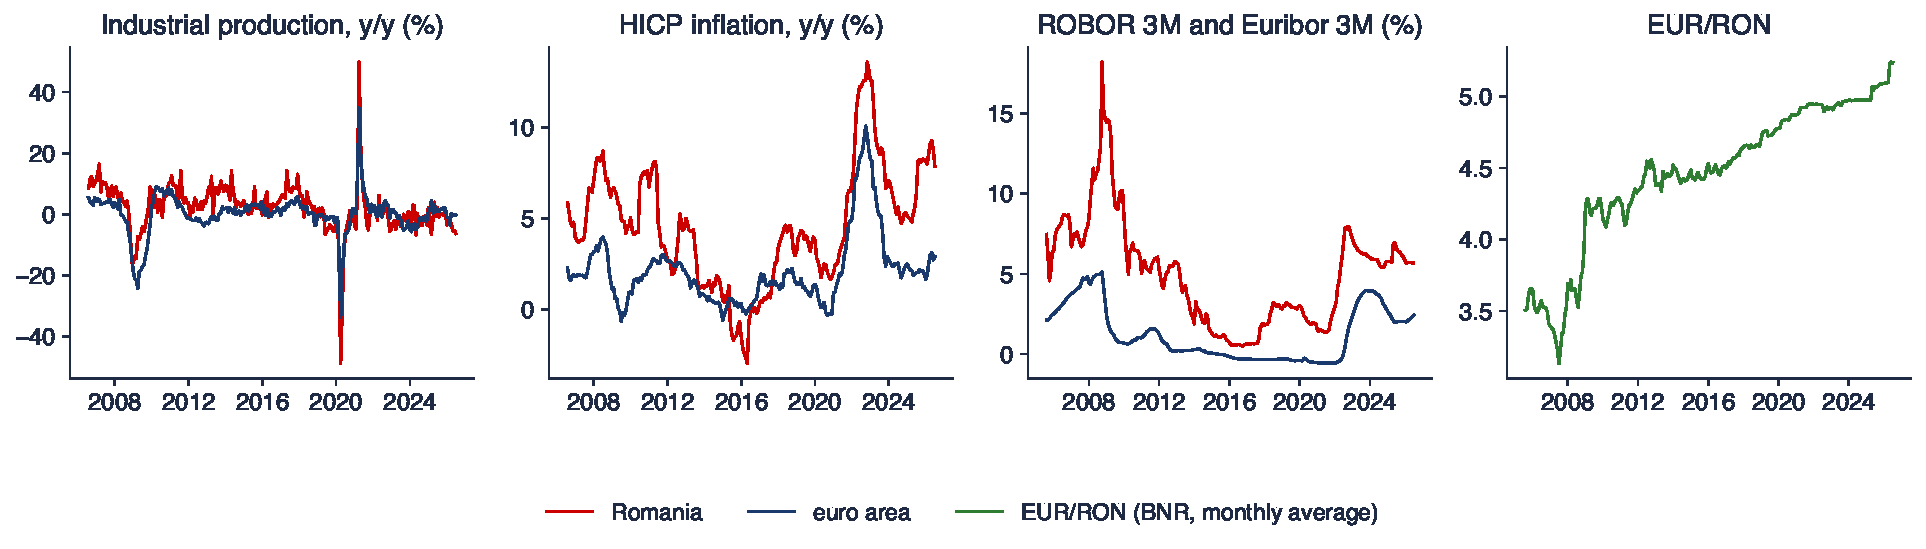
\includegraphics[width=0.97\textwidth,height=0.53\textheight,keepaspectratio]{ats_ch3_ro_data.pdf}
\end{center}
\vspace{-0.25cm}
\begin{itemize}
    \item Monthly, August 2005--July 2026: IP (SCA), HICP, 3-month money-market rates (Eurostat), EUR/RON (BNR reference rate, monthly average)
\end{itemize}
\quantlet{ATS\_ch3\_romania}{\qlurl{ATS_ch3_romania}}
\end{frame}

\begin{frame}{Interpreting the Romanian data}
\itemsize{\small}
\begin{itemize}
    \item HICP inflation peaked at 13.6\% in November 2022 and is 7.9\% in the last month; ROBOR 3M reached 18.2\% in the 2008 liquidity squeeze
    \item EUR/RON rose from 3.51 to 5.24: a trend depreciation with long managed-float plateaus
    \item Romanian and euro-area IP co-move closely, including the 2020 collapse: a strong case for an external block
    \item Sharp outliers (2008, 2020, 2022) will dominate the estimates of a small VAR: check robustness without them
\end{itemize}
\end{frame}

\begin{frame}{A VAR for Romania with a euro-area block}
\itemsize{\small}
\begin{itemize}
    \item $y_t$ = (EA IP, EA HICP, Euribor 3M, RO IP, RO HICP, ROBOR 3M, EUR/RON), logs $\times 100$ except rates; constant and monthly dummies (HICP is not seasonally adjusted)
    \begin{itemize}
        \item lag length: BIC and HQ choose 2, AIC 6; we use 2 ($T = 250$); largest root 1.006: levels, near-unit-root, no bias correction
    \end{itemize}
    \item Identification (Cholesky, in this order): the euro area does not react to Romania within the month; ROBOR reacts to Romanian activity and prices within the month; the exchange rate reacts to everything
    \begin{itemize}
        \item the zero restriction on the euro area is credible (Romania is small); the position of ROBOR before EUR/RON is debatable
        \item a block-exogenous VAR would also set the lagged Romanian effects on the euro area to zero (Seminar 3, B2 discusses orderings)
    \end{itemize}
\end{itemize}
\end{frame}

\begin{frame}{Responses to a domestic and a euro-area rate shock}
\itemsize{\footnotesize}
\begin{center}
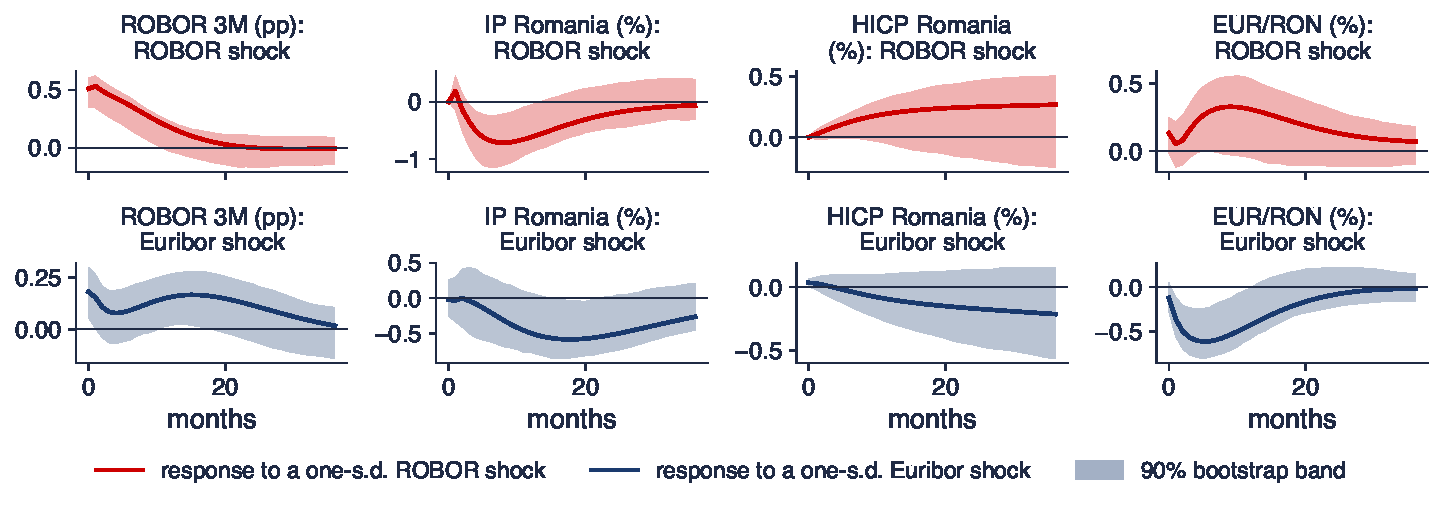
\includegraphics[width=0.97\textwidth,height=0.65\textheight,keepaspectratio]{ats_ch3_ro_var.pdf}
\end{center}
\vspace{-0.25cm}
\begin{itemize}
    \item VAR(2), Cholesky with the euro-area block first; one-standard-deviation shocks (ROBOR 0.51 pp, Euribor 0.09 pp); 90\% residual-bootstrap bands
\end{itemize}
\quantlet{ATS\_ch3\_romania}{\qlurl{ATS_ch3_romania}}
\end{frame}

\begin{frame}{Interpreting the Romanian responses}
\itemsize{\small}
\begin{itemize}
    \item ROBOR shock: IP \ensuremath{-}0.62\% after 12 months (band [\ensuremath{-}0.88, \ensuremath{-}0.06]); HICP 0.20\% (band [\ensuremath{-}0.06, 0.34]); EUR/RON 0.31\%
    \begin{itemize}
        \item a price puzzle and an exchange-rate puzzle (depreciation after a tightening): the ROBOR innovation still contains the BNR's reaction to inflation and to pressure on the leu
    \end{itemize}
    \item Euribor shock: Romanian IP \ensuremath{-}0.50\% after 12 months (band [\ensuremath{-}0.77, 0.07]); HICP \ensuremath{-}0.10\%; ROBOR 0.16 pp
    \item Honest summary: the recursive VAR identifies the euro-area block credibly and the domestic policy shock poorly
\end{itemize}
\end{frame}

\begin{frame}{The euro-area share of Romanian fluctuations}
\itemsize{\small}
\begin{center}
\scriptsize
\begin{tabular}{lrrrr}
\toprule
\textbf{Variable} & \textbf{EA shocks, 12 m} & \textbf{EA shocks, 36 m} & \textbf{ROBOR shock, 12 m} & \textbf{own shock, 12 m} \\
\midrule
IP Romania & 46\% & 37\% & 8\% & 41\% \\
HICP Romania & 44\% & 55\% & 3\% & 42\% \\
ROBOR 3M & 30\% & 39\% & 59\% & -- \\
EUR/RON & 25\% & 23\% & 6\% & 58\% \\
\bottomrule
\end{tabular}
\end{center}
\begin{itemize}
    \item Forecast error variance decomposition of the recursive VAR(2); EA shocks = the three euro-area shocks together
    \item Euro-area shocks explain 46\% of Romanian IP at one year and 55\% of HICP at three years; the domestic rate shock explains less than a tenth of either
    \item The shares are as credible as the ordering; with a block-exogenous VAR they are a lower bound for external influence
\end{itemize}
\end{frame}

\begin{frame}{ECB policy shocks and Romania: local projections}
\itemsize{\footnotesize}
\begin{center}
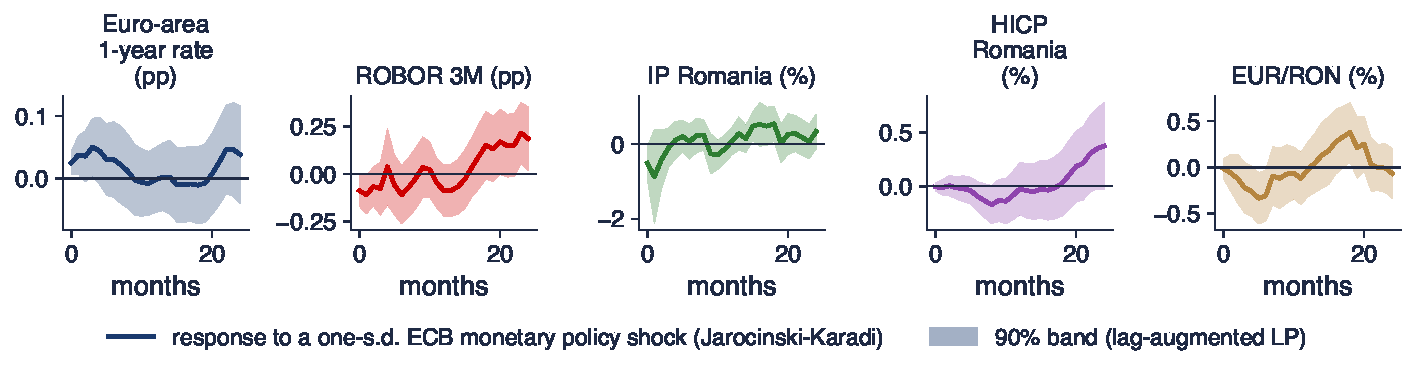
\includegraphics[width=0.97\textwidth,height=0.48\textheight,keepaspectratio]{ats_ch3_ro_lp.pdf}
\end{center}
\vspace{-0.25cm}
\begin{itemize}
    \item Shock: the pure monetary policy shock of \refJK\ (authors' update, one s.d. = 3.2 bp); 3 lags of all variables and of the shock (lag augmentation), monthly dummies; origins 2005:8--2025:10
\end{itemize}
\quantlet{ATS\_ch3\_romania}{\qlurl{ATS_ch3_romania}}
\end{frame}

\begin{frame}{Interpreting the spillover projections}
\itemsize{\small}
\begin{itemize}
    \item Relevance first: the euro-area 1-year rate rises by 0.03 pp on impact (SE 0.01); first-stage $F = 4.8$ (impact) and 4.0 (one month)
    \begin{itemize}
        \item monthly averages dilute an announcement-day surprise: the shock is a weak instrument for monthly euro-area rates
    \end{itemize}
    \item Romanian HICP: \ensuremath{-}0.02\% after 12 months (SE 0.15), 0.37\% after 24 (SE 0.25); EUR/RON \ensuremath{-}0.31\% after 6 months (SE 0.17)
    \item Honest conclusion: with a weak external shock and 20 years of data, the spillovers to Romanian prices are not determined; a weak-IV-robust set is wide (Seminar 3, C1)
\end{itemize}
\end{frame}

\begin{frame}{Conclusions for Romania}
\itemsize{\small}
\begin{itemize}
    \item Robust findings
    \begin{itemize}
        \item euro-area shocks account for a large share of Romanian output and price fluctuations
        \item a euro-area tightening lowers Romanian IP within a year in the recursive VAR
    \end{itemize}
    \item Fragile findings
    \begin{itemize}
        \item the effect of a domestic ROBOR shock on prices and the leu: puzzles signal an identification failure, not a fact about Romania
        \item the size of ECB spillovers to Romanian inflation: the instrument is weak at a monthly frequency
    \end{itemize}
    \item Next steps (projects)
    \begin{itemize}
        \item BNR policy-meeting surprises from ROBOR or FRA quotes around announcements, used as a proxy
        \item sign restrictions (a tightening appreciates the leu and lowers prices) and a Bayesian VAR with shrinkage (\atschlink{https://danpele.github.io/Advanced-Time-Series/EN/Courses/chapter5_bvar_factor_models_nowcasting.pdf}{Chapter 5})
    \end{itemize}
\end{itemize}
\end{frame}

\begin{frame}{Recap: Romania and euro-area spillovers}
\itemsize{\small}
\begin{itemize}
    \item Put the large neighbour first: the euro-area block is credibly exogenous within the month
    \item A recursive ROBOR shock produces price and exchange-rate puzzles
    \item External ECB shocks are weak instruments at a monthly frequency: report the uncertainty, do not hide it
\end{itemize}
\end{frame}


%=============================================================================
\section{AI for scientific discovery}
%=============================================================================

\begin{frame}{An open question}
\itemsize{\small}
\begin{itemize}
    \item How strongly does ECB monetary policy pass through to Romanian inflation, and has the pass-through changed since 2022?
    \begin{itemize}
        \item formal: $H_0$: $\theta_{12} = 0$, the 12-month response of Romanian HICP to a 25 bp euro-area rate shock, tested by an Anderson--Rubin set that is valid with weak instruments
        \item falsified by a bounded 90\% set that excludes zero for a pre-registered shock, horizon and sample
    \end{itemize}
    \item Why it matters: Romania plans to join the euro area; the BNR needs to know how much of its inflation is imported
    \begin{itemize}
        \item literature to start from: \refJK, \refSWc, \refMSW, \refPW, \refLPW
    \end{itemize}
\end{itemize}
\end{frame}

\begin{frame}{The discovery loop with an AI assistant}
\itemsize{\footnotesize}
\begin{itemize}
    \item An AI assistant (an LLM such as Claude, ChatGPT, Gemini or Copilot) speeds up each step; Semantic Scholar and Elicit help with the literature
    \begin{itemize}
        \item \textbf{literature}: \aiprompt{List peer-reviewed papers that estimate euro-area monetary spillovers to Romania or Central and Eastern Europe with high-frequency shocks; give DOIs.} Then check every DOI on Crossref
        \item \textbf{hypothesis}: \aiprompt{Propose three channels (trade, exchange rate, bank funding) and one observable implication of each.}
        \item \textbf{code and replication}: ask for an LP-IV function, then reproduce a known number first (the first-stage $F$ of this lecture)
        \item \textbf{robustness and critique}: \aiprompt{Act as a hostile referee: list every way this identification of ECB spillovers could fail.}
    \end{itemize}
    \item Report: what was asked, what was kept, what was rejected (AI\_USE.md, AI\_ERRORS.md)
\end{itemize}
\end{frame}

\begin{frame}{Required checks}
\itemsize{\small}
\begin{itemize}
    \item Every reference exists and says what is claimed (DOI resolves, title matches, the result is in the paper)
    \item The shock is dated correctly: announcement-day surprises are summed within the month, never shifted forward
    \item Relevance is reported (first-stage $F$ with HAC variance) before any response is interpreted
    \item Lags, horizons, sample and the treatment of 2020 are fixed before the results; all variants are reported
    \item An AI summary of a ``significant spillover'' is checked against the confidence set, not against the point estimate
\end{itemize}
\end{frame}

\begin{frame}{Mini-case: the robustness of one number}
\itemsize{\footnotesize}
\begin{center}
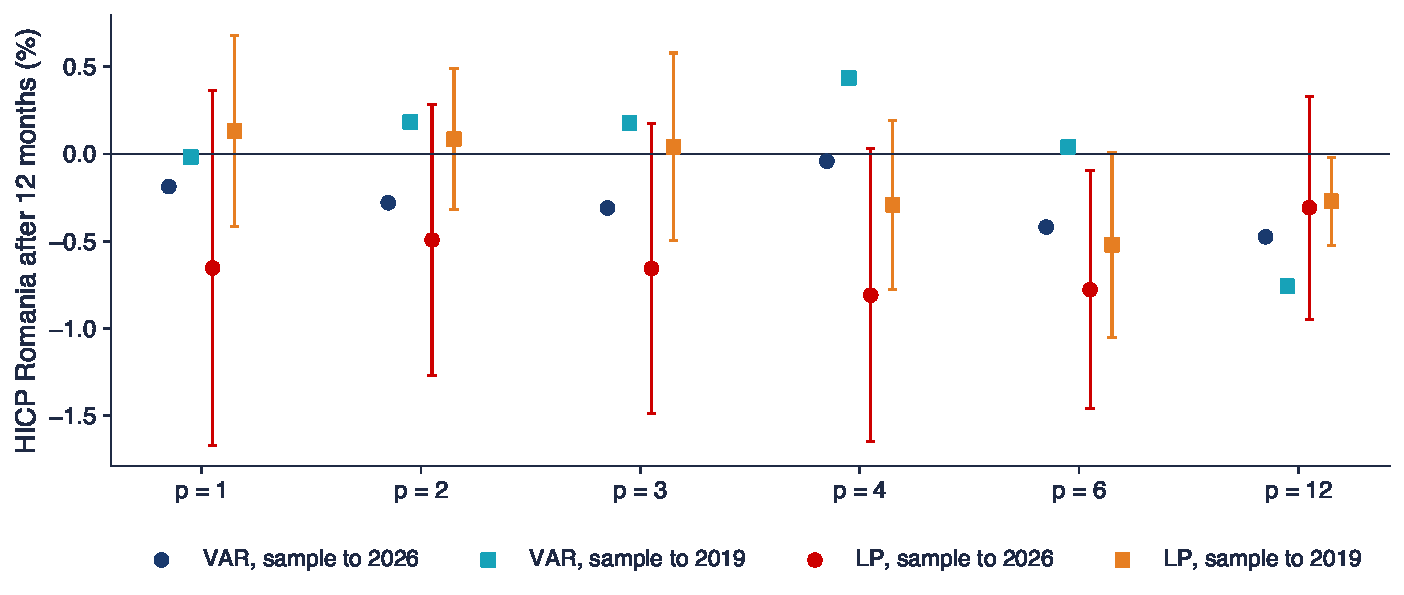
\includegraphics[width=0.97\textwidth,height=0.55\textheight,keepaspectratio]{ats_ch3_ai_case.pdf}
\end{center}
\vspace{-0.25cm}
\begin{itemize}
    \item Response of Romanian HICP after 12 months to a 25 bp Euribor shock: recursive VAR and recursive LP (90\% Newey--West bars), lag length $p$, samples ending in 2019 and in 2026
    \item 24 estimates range from \ensuremath{-}0.81\% to 0.44\%, 7 of them positive: the sign depends on the lag length and on the post-2020 data; an AI assistant that reports one of them ``with confidence'' is wrong
\end{itemize}
\quantlet{ATS\_ch3\_romania}{\qlurl{ATS_ch3_romania}}
\end{frame}

\begin{frame}{Project idea}
\itemsize{\small}
\begin{itemize}
    \item \textbf{Euro-area monetary spillovers to Romania}: replicate first, then extend
    \begin{itemize}
        \item replicate: the proxy SVAR of \refGK\ (this lecture: $F = 17.7$, the bond-premium jump) and the Romanian LP of this lecture
        \item extend: daily ECB surprises aggregated to monthly with the Gertler--Karadi averaging; a quarterly GDP version; Anderson--Rubin sets; sign restrictions on the surprises (\refJK)
        \item pre-register: shock, outcomes, horizons 0--24, lag rule, the 2020 treatment and the Holm correction across outcomes
    \end{itemize}
    \item Deliverables follow the course rules: repository, report, AI\_USE.md, AI\_ERRORS.md, oral defence
\end{itemize}
\end{frame}


%=============================================================================
\section{Wrap-up}
%=============================================================================

\begin{frame}{Key takeaways}
\itemsize{\small}
\begin{itemize}
    \item A structural VAR is a reduced form plus an identifying assumption; the assumption is the economics
    \item Zeros (short or long run), signs, narratives, heteroskedasticity and instruments each buy identification with a different assumption
    \item Set identification is honest: report the set and the role of the prior
    \item Inference: bootstrap matched to the setting, bias correction, joint bands, weak-IV-robust sets
    \item LP and VAR estimate the same responses; choose by bias and variance, and use LP for state dependence
\end{itemize}
\end{frame}

\begin{frame}{Self-assessment}
\itemsize{\small}
\begin{columns}[T]
\begin{column}{0.56\textwidth}
\begin{block}{Questions}
\begin{itemize}
    \item How many restrictions identify a five-variable SVAR exactly?
    \item Why does $\E u_tz_t$ identify the impact column of a proxy SVAR?
    \item What does the posterior median of a sign-restricted response fail to represent?
    \item When does a VAR beat LP in mean squared error?
    \item Why is the wild bootstrap invalid for a proxy SVAR?
\end{itemize}
\end{block}
\end{column}
\begin{column}{0.40\textwidth}
\begin{block}{Next: \atschlink{https://danpele.github.io/Advanced-Time-Series/EN/Courses/chapter4_cointegration_vecm_ardl_panel.pdf}{Chapter 4}}
\begin{itemize}
    \item Cointegration revisited: VECM, ARDL and panel data
    \item Long-run restrictions become restrictions on cointegrating vectors and on the common trends
\end{itemize}
\end{block}
\end{column}
\end{columns}
\end{frame}


%=============================================================================
\section{Appendix}
%=============================================================================

\begin{frame}{Appendix: the long-run restriction in closed form}
\hypertarget{atsapp1}{}\atsappback{atssrc1}{Back}
\itemsize{\small}
\begin{itemize}
    \item Stable VAR: $\sum_{h\ge0}\Phi_h = A(1)^{-1}$, so the long-run response matrix is $\Theta(1) = A(1)^{-1}B_0$
    \item $\Theta(1)\Theta(1)' = A(1)^{-1}B_0B_0'A(1)^{-1\prime} = A(1)^{-1}\Sigma_uA(1)^{-1\prime}$, known from the reduced form
    \item $[\Theta(1)]_{12} = 0$ makes $\Theta(1)$ lower triangular: $\Theta(1) = \mathrm{chol}(A(1)^{-1}\Sigma_uA(1)^{-1\prime})$, unique with a positive diagonal
    \item Hence $B_0 = A(1)\Theta(1)$; check $B_0B_0' = \Sigma_u$; signs are then normalised (supply raises output in the long run)
\end{itemize}
\end{frame}

\begin{frame}{Appendix: identifying the column $b_1$ with a proxy}
\hypertarget{atsapp2}{}\atsappback{atssrc2}{Back}
\itemsize{\small}
\begin{itemize}
    \item $u_t = B_0\varepsilon_t = b_1\varepsilon_{1t} + \sum_{j\ge2}b_j\varepsilon_{jt}$
    \item $\E u_tz_t = b_1\E\varepsilon_{1t}z_t + \sum_{j\ge2}b_j\E\varepsilon_{jt}z_t = \alpha b_1$ by exogeneity
    \item Relative impacts $b_{i1}/b_{11} = \E u_{it}z_t/\E u_{1t}z_t$ need $\alpha \ne 0$ (relevance); the scale of $b_1$ follows from $b_1'\Sigma_u^{-1}b_1 = 1$
\end{itemize}
\end{frame}

\begin{frame}{Appendix: LP and VAR agree up to horizon $p$}
\hypertarget{atsapp3}{}\atsappback{atssrc3}{Back}
\itemsize{\small}
\begin{itemize}
    \item Let $w_t = (y_{t-1}, \dots, y_{t-p})$ and the shock be the innovation $\tilde x_t = x_t - \mathrm{proj}(x_t\mid w_t)$
    \item LP coefficient: $\beta_h = \Cov(y_{t+h}, \tilde x_t)/\Var(\tilde x_t)$ (Frisch--Waugh)
    \item The VAR($p$) reproduces the autocovariances $\Gamma_0, \dots, \Gamma_p$ exactly; for $h \le p$, $\Cov(y_{t+h}, \tilde x_t)$ depends only on them, so both give the same $\beta_h$ \refPW
    \item For $h > p$ the VAR extrapolates its own autocovariances: the source of the bias of a short VAR, and of the lower variance
\end{itemize}
\end{frame}


%=============================================================================
\section{References}
%=============================================================================

\begin{frame}{References (1/4)}
\itemsize{\tiny}
\begin{itemize}
    \item Antolín-Díaz, J., \& Rubio-Ramírez, J. F. (2018). Narrative sign restrictions for SVARs. \textit{American Economic Review}, 108(10), 2802--2829. \href{https://doi.org/10.1257/aer.20161852}{doi:10.1257/aer.20161852}
    \item Arias, J. E., Rubio-Ramírez, J. F., \& Waggoner, D. F. (2018). Inference based on structural vector autoregressions identified with sign and zero restrictions: Theory and applications. \textit{Econometrica}, 86(2), 685--720. \href{https://doi.org/10.3982/ECTA14468}{doi:10.3982/ECTA14468}
    \item Bauer, M. D., \& Swanson, E. T. (2023). A reassessment of monetary policy surprises and high-frequency identification. \textit{NBER Macroeconomics Annual}, 37, 87--155. \href{https://doi.org/10.1086/723574}{doi:10.1086/723574}
    \item Baumeister, C., \& Hamilton, J. D. (2015). Sign restrictions, structural vector autoregressions, and useful prior information. \textit{Econometrica}, 83(5), 1963--1999. \href{https://doi.org/10.3982/ECTA12356}{doi:10.3982/ECTA12356}
    \item Baumeister, C., \& Hamilton, J. D. (2019). Structural interpretation of vector autoregressions with incomplete identification: Revisiting the role of oil supply and demand shocks. \textit{American Economic Review}, 109(5), 1873--1910. \href{https://doi.org/10.1257/aer.20151569}{doi:10.1257/aer.20151569}
    \item Blanchard, O. J., \& Quah, D. (1989). The dynamic effects of aggregate demand and supply disturbances. \textit{American Economic Review}, 79(4), 655--673. \href{https://www.jstor.org/stable/1827924}{jstor.org}
    \item Blanchard, O., \& Perotti, R. (2002). An empirical characterization of the dynamic effects of changes in government spending and taxes on output. \textit{The Quarterly Journal of Economics}, 117(4), 1329--1368. \href{https://doi.org/10.1162/003355302320935043}{doi:10.1162/003355302320935043}
    \item Christiano, L. J., Eichenbaum, M., \& Evans, C. L. (1999). Monetary policy shocks: What have we learned and to what end? In J. B. Taylor \& M. Woodford (Eds.), \textit{Handbook of Macroeconomics} (Vol.\ 1A, pp.\ 65--148). Elsevier. \href{https://doi.org/10.1016/S1574-0048(99)01005-8}{doi:10.1016/S1574-0048(99)01005-8}
    \item Faust, J., \& Leeper, E. M. (1997). When do long-run identifying restrictions give reliable results? \textit{Journal of Business \& Economic Statistics}, 15(3), 345--353. \href{https://doi.org/10.1080/07350015.1997.10524712}{doi:10.1080/07350015.1997.10524712}
    \item Fry, R., \& Pagan, A. (2011). Sign restrictions in structural vector autoregressions: A critical review. \textit{Journal of Economic Literature}, 49(4), 938--960. \href{https://doi.org/10.1257/jel.49.4.938}{doi:10.1257/jel.49.4.938}
    \item Galí, J. (1999). Technology, employment, and the business cycle: Do technology shocks explain aggregate fluctuations? \textit{American Economic Review}, 89(1), 249--271. \href{https://doi.org/10.1257/aer.89.1.249}{doi:10.1257/aer.89.1.249}
\end{itemize}
\end{frame}

\begin{frame}{References (2/4)}
\itemsize{\tiny}
\begin{itemize}
    \item Gertler, M., \& Karadi, P. (2015). Monetary policy surprises, credit costs, and economic activity. \textit{American Economic Journal: Macroeconomics}, 7(1), 44--76. \href{https://doi.org/10.1257/mac.20130329}{doi:10.1257/mac.20130329}
    \item Giacomini, R., \& Kitagawa, T. (2021). Robust Bayesian inference for set-identified models. \textit{Econometrica}, 89(4), 1519--1556. \href{https://doi.org/10.3982/ecta16773}{doi:10.3982/ecta16773}
    \item Gilchrist, S., \& Zakrajšek, E. (2012). Credit spreads and business cycle fluctuations. \textit{American Economic Review}, 102(4), 1692--1720. \href{https://doi.org/10.1257/aer.102.4.1692}{doi:10.1257/aer.102.4.1692}
    \item Gonçalves, S., \& Kilian, L. (2004). Bootstrapping autoregressions with conditional heteroskedasticity of unknown form. \textit{Journal of Econometrics}, 123(1), 89--120. \href{https://doi.org/10.1016/j.jeconom.2003.10.030}{doi:10.1016/j.jeconom.2003.10.030}
    \item Gürkaynak, R. S., Sack, B., \& Swanson, E. T. (2005). Do actions speak louder than words? The response of asset prices to monetary policy actions and statements. \textit{International Journal of Central Banking}, 1(1), 55--93. \href{https://www.ijcb.org/journal/ijcb05q2a2.htm}{ijcb.org}
    \item Hamilton, J. D. (1994). \textit{Time Series Analysis}. Princeton University Press. \href{https://doi.org/10.2307/j.ctv14jx6sm}{doi:10.2307/j.ctv14jx6sm}
    \item Jarociński, M., \& Karadi, P. (2020). Deconstructing monetary policy surprises: The role of information shocks. \textit{American Economic Journal: Macroeconomics}, 12(2), 1--43. \href{https://doi.org/10.1257/mac.20180090}{doi:10.1257/mac.20180090}
    \item Jentsch, C., \& Lunsford, K. G. (2019). The dynamic effects of personal and corporate income tax changes in the United States: Comment. \textit{American Economic Review}, 109(7), 2655--2678. \href{https://doi.org/10.1257/aer.20162011}{doi:10.1257/aer.20162011}
    \item Jordà, Ò. (2005). Estimation and inference of impulse responses by local projections. \textit{American Economic Review}, 95(1), 161--182. \href{https://doi.org/10.1257/0002828053828518}{doi:10.1257/0002828053828518}
    \item Kilian, L., \& Lütkepohl, H. (2017). \textit{Structural Vector Autoregressive Analysis}. Cambridge University Press. \href{https://doi.org/10.1017/9781108164818}{doi:10.1017/9781108164818}
    \item Kilian, L. (2019). Measuring global real economic activity: Do recent critiques hold up to scrutiny? \textit{Economics Letters}, 178, 106--110. \href{https://doi.org/10.1016/j.econlet.2019.03.001}{doi:10.1016/j.econlet.2019.03.001}
\end{itemize}
\end{frame}

\begin{frame}{References (3/4)}
\itemsize{\tiny}
\begin{itemize}
    \item Kilian, L. (2009). Not all oil price shocks are alike: Disentangling demand and supply shocks in the crude oil market. \textit{American Economic Review}, 99(3), 1053--1069. \href{https://doi.org/10.1257/aer.99.3.1053}{doi:10.1257/aer.99.3.1053}
    \item Kilian, L. (1998). Small-sample confidence intervals for impulse response functions. \textit{The Review of Economics and Statistics}, 80(2), 218--230. \href{https://doi.org/10.1162/003465398557465}{doi:10.1162/003465398557465}
    \item Kuttner, K. N. (2001). Monetary policy surprises and interest rates: Evidence from the Fed funds futures market. \textit{Journal of Monetary Economics}, 47(3), 523--544. \href{https://doi.org/10.1016/S0304-3932(01)00055-1}{doi:10.1016/S0304-3932(01)00055-1}
    \item Lanne, M., \& Lütkepohl, H. (2008). Identifying monetary policy shocks via changes in volatility. \textit{Journal of Money, Credit and Banking}, 40(6), 1131--1149. \href{https://doi.org/10.1111/j.1538-4616.2008.00151.x}{doi:10.1111/j.1538-4616.2008.00151.x}
    \item Li, D., Plagborg-Møller, M., \& Wolf, C. K. (2024). Local projections vs.\ VARs: Lessons from thousands of DGPs. \textit{Journal of Econometrics}, 244(2), 105722. \href{https://doi.org/10.1016/j.jeconom.2024.105722}{doi:10.1016/j.jeconom.2024.105722}
    \item Lütkepohl, H. (2005). \textit{New Introduction to Multiple Time Series Analysis}. Springer. \href{https://doi.org/10.1007/978-3-540-27752-1}{doi:10.1007/978-3-540-27752-1}
    \item Mertens, K., \& Ravn, M. O. (2013). The dynamic effects of personal and corporate income tax changes in the United States. \textit{American Economic Review}, 103(4), 1212--1247. \href{https://doi.org/10.1257/aer.103.4.1212}{doi:10.1257/aer.103.4.1212}
    \item Montiel Olea, J. L., \& Plagborg-Møller, M. (2021). Local projection inference is simpler and more robust than you think. \textit{Econometrica}, 89(4), 1789--1823. \href{https://doi.org/10.3982/ECTA18756}{doi:10.3982/ECTA18756}
    \item Montiel Olea, J. L., \& Plagborg-Møller, M. (2019). Simultaneous confidence bands: Theory, implementation, and an application to SVARs. \textit{Journal of Applied Econometrics}, 34(1), 1--17. \href{https://doi.org/10.1002/jae.2656}{doi:10.1002/jae.2656}
    \item Montiel Olea, J. L., Stock, J. H., \& Watson, M. W. (2021). Inference in structural vector autoregressions identified with an external instrument. \textit{Journal of Econometrics}, 225(1), 74--87. \href{https://doi.org/10.1016/j.jeconom.2020.05.014}{doi:10.1016/j.jeconom.2020.05.014}
    \item Nakamura, E., \& Steinsson, J. (2018). High-frequency identification of monetary non-neutrality: The information effect. \textit{The Quarterly Journal of Economics}, 133(3), 1283--1330. \href{https://doi.org/10.1093/qje/qjy004}{doi:10.1093/qje/qjy004}
\end{itemize}
\end{frame}

\begin{frame}{References (4/4)}
\itemsize{\tiny}
\begin{itemize}
    \item Plagborg-Møller, M., \& Wolf, C. K. (2021). Local projections and VARs estimate the same impulse responses. \textit{Econometrica}, 89(2), 955--980. \href{https://doi.org/10.3982/ECTA17813}{doi:10.3982/ECTA17813}
    \item Ramey, V. A. (2016). Macroeconomic shocks and their propagation. In J. B. Taylor \& H. Uhlig (Eds.), \textit{Handbook of Macroeconomics} (Vol.\ 2A, pp.\ 71--162). Elsevier. \href{https://doi.org/10.1016/bs.hesmac.2016.03.003}{doi:10.1016/bs.hesmac.2016.03.003}
    \item Ramey, V. A., \& Zubairy, S. (2018). Government spending multipliers in good times and in bad: Evidence from US historical data. \textit{Journal of Political Economy}, 126(2), 850--901. \href{https://doi.org/10.1086/696277}{doi:10.1086/696277}
    \item Rigobon, R. (2003). Identification through heteroskedasticity. \textit{The Review of Economics and Statistics}, 85(4), 777--792. \href{https://doi.org/10.1162/003465303772815727}{doi:10.1162/003465303772815727}
    \item Romer, C. D., \& Romer, D. H. (2004). A new measure of monetary shocks: Derivation and implications. \textit{American Economic Review}, 94(4), 1055--1084. \href{https://doi.org/10.1257/0002828042002651}{doi:10.1257/0002828042002651}
    \item Rubio-Ramírez, J. F., Waggoner, D. F., \& Zha, T. (2010). Structural vector autoregressions: Theory of identification and algorithms for inference. \textit{The Review of Economic Studies}, 77(2), 665--696. \href{https://doi.org/10.1111/j.1467-937X.2009.00578.x}{doi:10.1111/j.1467-937X.2009.00578.x}
    \item Sims, C. A. (1980). Macroeconomics and reality. \textit{Econometrica}, 48(1), 1--48. \href{https://doi.org/10.2307/1912017}{doi:10.2307/1912017}
    \item Stock, J. H., \& Watson, M. W. (2012). Disentangling the channels of the 2007--09 recession. \textit{Brookings Papers on Economic Activity}, 2012(1), 81--135. \href{https://doi.org/10.1353/eca.2012.0005}{doi:10.1353/eca.2012.0005}
    \item Stock, J. H., \& Watson, M. W. (2018). Identification and estimation of dynamic causal effects in macroeconomics using external instruments. \textit{The Economic Journal}, 128(610), 917--948. \href{https://doi.org/10.1111/ecoj.12593}{doi:10.1111/ecoj.12593}
    \item Stock, J. H., \& Watson, M. W. (2001). Vector autoregressions. \textit{Journal of Economic Perspectives}, 15(4), 101--115. \href{https://doi.org/10.1257/jep.15.4.101}{doi:10.1257/jep.15.4.101}
    \item Uhlig, H. (2005). What are the effects of monetary policy on output? Results from an agnostic identification procedure. \textit{Journal of Monetary Economics}, 52(2), 381--419. \href{https://doi.org/10.1016/j.jmoneco.2004.05.007}{doi:10.1016/j.jmoneco.2004.05.007}
\end{itemize}
\end{frame}

\end{document}
